\documentclass[11pt]{beamer}
\title[Multirate Digital Signal Processing and Adaptive Filter Banks]{Confronto fra algoritmo LMS e Fast Deconvolution per la cancellazione del crosstalk}
\author{Matteo Orlandini e Jacopo Pagliuca}
\date{\today}
\institute[UnivPM]{Universit� Politecnica delle Marche}
%\logo{\includegraphics[width=15mm]{Immagini/univpmlogo}}
\titlegraphic{
\includegraphics[width=2cm]{Immagini/univpmlogo}
}
\usepackage[english, italian]{babel} %l?ultima lingua dichiarata � la lingua principale del documento
\usepackage[latin1]{inputenc}
\usepackage[T1]{fontenc}
%\usepackage{subfig}
\usepackage{graphicx}
\usepackage{animate} %per le gif 
\usepackage{xcolor}
\usepackage{listings}
\usepackage{siunitx}
\usepackage{booktabs} %toprule, midrule, bottomrule
\usepackage{subcaption,booktabs}

\usetheme{Antibes}
\usecolortheme{default} %https://hartwork.org/beamer-theme-matrix/
%\useoutertheme[right,color=red]{sidebar} %{infolines}
%\setbeamertemplate{sidebar canvas right}[vertical shading][top=red,bottom=white]
\setbeamercovered{dynamic}

%\usepackage[latin1]{inputenc} %l'ho messo io (Jacopo)
%inizio impostazioni bibliografia
\usepackage[autostyle,italian=guillemets]{csquotes} 
%autostyle adatta lo stile delle citazioni alla lingua corrente del documento;
%italian=guillemets racchiude automaticamente tra virgolette caporali
%i campi che prevedono le virgolette;
\usepackage[backend=biber, style=numeric, citestyle=numeric,maxcitenames=2,maxbibnames = 2]{biblatex}
%backend=biber dice a biblatex che s?intende usare Biber come motore bibliografico
%style:numeric Anno di pubblicazione: in fondo al riferimento.
%citestyle=numeric Riferimento: numerico ([1], [2], eccetera).
%fine impostazioni bibliografia
\renewcommand*{\bibfont}{\footnotesize}

\addbibresource{Bibliografia.bib}

\begin{document}
	\begin{frame}
		\maketitle
	\end{frame}

\begin{frame}
	\frametitle{Contenuti}
	\tableofcontents
\end{frame}

\section{Introduzione}
\begin{frame}
\tableofcontents[currentsection]
\end{frame}

\begin{frame}
\frametitle{Cancellazione del crosstalk}
	\begin{block}{Obiettivo}
		Confrontare gli algoritmi LMS e Fast Deconvolution per la cancellazione del crosstalk.
	\end{block}
\begin{itemize}
\item Un sistema audio 3D permette
di posizionare i suoni intorno ad un ascoltatore in modo che questi siano
percepiti come provenienti da punti arbitrari nello spazio.
\item Se vengono utilizzati degli altoparlanti, la riproduzione di segnali binaurali all'orecchio dell'ascoltatore non � semplice. Ogni orecchio riceve una componente di diafonia, inoltre, i segnali diretti sono distorti dal riverbero della stanza. 
\item Per superare i problemi descritti sopra, � necessario un filtro
inverso prima di riprodurre il segnale binaurale attraverso gli altoparlanti.
\end{itemize}
\end{frame}

\section{Stato dell'arte}
\begin{frame}
\tableofcontents[currentsection]
\end{frame}

\begin{frame}
\frametitle{Algoritmi adattativi}
\end{frame}	

\begin{frame}
\frametitle{Algoritmi nel dominio della frequenza}
\end{frame}	
	
\section{Dataset}
\begin{frame}
\tableofcontents[currentsection]
\end{frame}

\begin{frame}
\frametitle{Dataset utilizzato}
\begin{block}{HRTF Measurements of a KEMAR Dummy-Head Microphone}%~\cite{Gardner:HRTF}
\begin{itemize}
\item Dataset del MIT.
\item Risposte impulsive dell'orecchio sinistro
e destro di un altoparlante Realistic Optimus Pro 7 montato a 1,4 metri dal
KEMAR.
\item I dati HRTF vengono archiviati nelle directory per elevazione. Ogni nome
di directory ha il formato ``elevEE'', dove ``EE'' � l'angolo di elevazione.
\item All'interno
di ogni directory, il nome di ogni file ha il formato ``XEEeAAAa.wav''
dove X pu� essere ``L'' o ``R'' rispettivamente per la risposta dell'orecchio
sinistro e destro e ``AAA'' � l'azimut della sorgente in gradi, da 0� a 355�.
\end{itemize}
\end{block}
\end{frame}	

\section{LMS}
\begin{frame}
\tableofcontents[currentsection]
\end{frame}

\section{Fast Deconvolution}
\begin{frame}
\tableofcontents[currentsection]
\end{frame}

\section{Risultati}
\begin{frame}
\tableofcontents[currentsection]
\end{frame}

\begin{frame}{Risultati Matlab}
\begin{block}{Fattori di separazione dei canali}
\begin{equation}\label{eq:JL}
J_L = E\left\{20\cdot\log_{10} \dfrac{C_{11}H_{11}+C_{12}H_{21}}{C_{21}H_{11}+C_{22}H_{21}}\right\} \quad [\si{\decibel}]
\end{equation}

\begin{equation}\label{eq:JR}
J_R = E\left\{20\cdot\log_{10} \dfrac{C_{22}H_{22}+C_{21}H_{12}}{C_{12}H_{22}+C_{11}H_{12}}\right\} \quad [\si{\decibel}]
\end{equation}
\end{block}
\end{frame}

\begin{frame}
\begin{table}[h]
    \begin{subtable}{.4\linewidth}
      \centering
        \begin{tabular}{c c c}
        \toprule
        $\mu$   & $J_R$ [\si{\decibel}]   & $J_L$ [\si{\decibel}]   \\ \midrule
        $10^{-3}$ & 22.032 & 21.924 \\
        $5\cdot10^{-4}$ & 17.610 & 20.375 \\
        $10^{-4}$& 11.063 & 16.921 \\
        $5\cdot10^{-5}$ & 9.742  & 16.161 \\ \bottomrule
        \end{tabular}
        \caption{\label{tab:LMS_result}Confronto di $J_R$ e $J_L$ per l'algoritmo LMS per diversi $\mu$.}
    \end{subtable}
    \hfill
    \begin{subtable}{.4\linewidth}
      \centering
        \begin{tabular}{c c c}
        \toprule
		$\beta$   & $J_R$ [\si{\decibel}]   & $J_L$ [\si{\decibel}]   \\ \midrule
		$1$ &  25.062 &  26.538\\
		$0.3$ &  28.829 &  30.498\\
		$0.1$&  34.908 & 36.532 \\
		$0.01$ &  47.657 &  48.661 \\ \bottomrule
        \end{tabular}
		\caption{\label{tab:FD_result}Confronto di $J_R$ e $J_L$ per l'algoritmo FD per diversi $\beta$.}
    \end{subtable} 
    \vfill
     \begin{subtable}{.4\linewidth}
          \centering
            \begin{tabular}{c c c}
            \toprule
            Azimuth  & $J_R$ [\si{\decibel}]   & $J_L$ [\si{\decibel}]   \\ \midrule
            $\pm \SI{20}{\degree}$ & 21.511 & 25.532\\
            $\pm \SI{30}{\degree}$ & 22.032 & 21.924  \\
            $\pm \SI{40}{\degree}$ & 19.667 & 23.528 \\ \bottomrule
            \end{tabular}
            \caption{\label{tab:LMS_result_azimuth}Confronto di $J_R$ e $J_L$ per l'algoritmo LMS per diversi angoli azimutali con $\mu = 10^{-3}$.}
    \end{subtable}
 	\hfill 
     \begin{subtable}{.4\linewidth}
        \centering
          \begin{tabular}{c c c}
          \toprule
          Azimuth  & $J_R$ [\si{\decibel}]   & $J_L$ [\si{\decibel}]   \\ \midrule
          $\pm \SI{20}{\degree}$ &  45.672 &  47.034\\
          $\pm \SI{30}{\degree}$ &  34.908 & 36.532 \\
          $\pm \SI{40}{\degree}$ &  40.523 &  42.098\\ \bottomrule
          \end{tabular}
          \caption{\label{tab:FD_result_azimuth}Confronto di $J_R$ e $J_L$ per l'algoritmo FD per diversi angoli azimutali con $\beta = 0.1$.}
      \end{subtable}
\end{table}
\end{frame}

\begin{frame}
\begin{figure}[h]
\begin{subfigure}{.45\textwidth}
	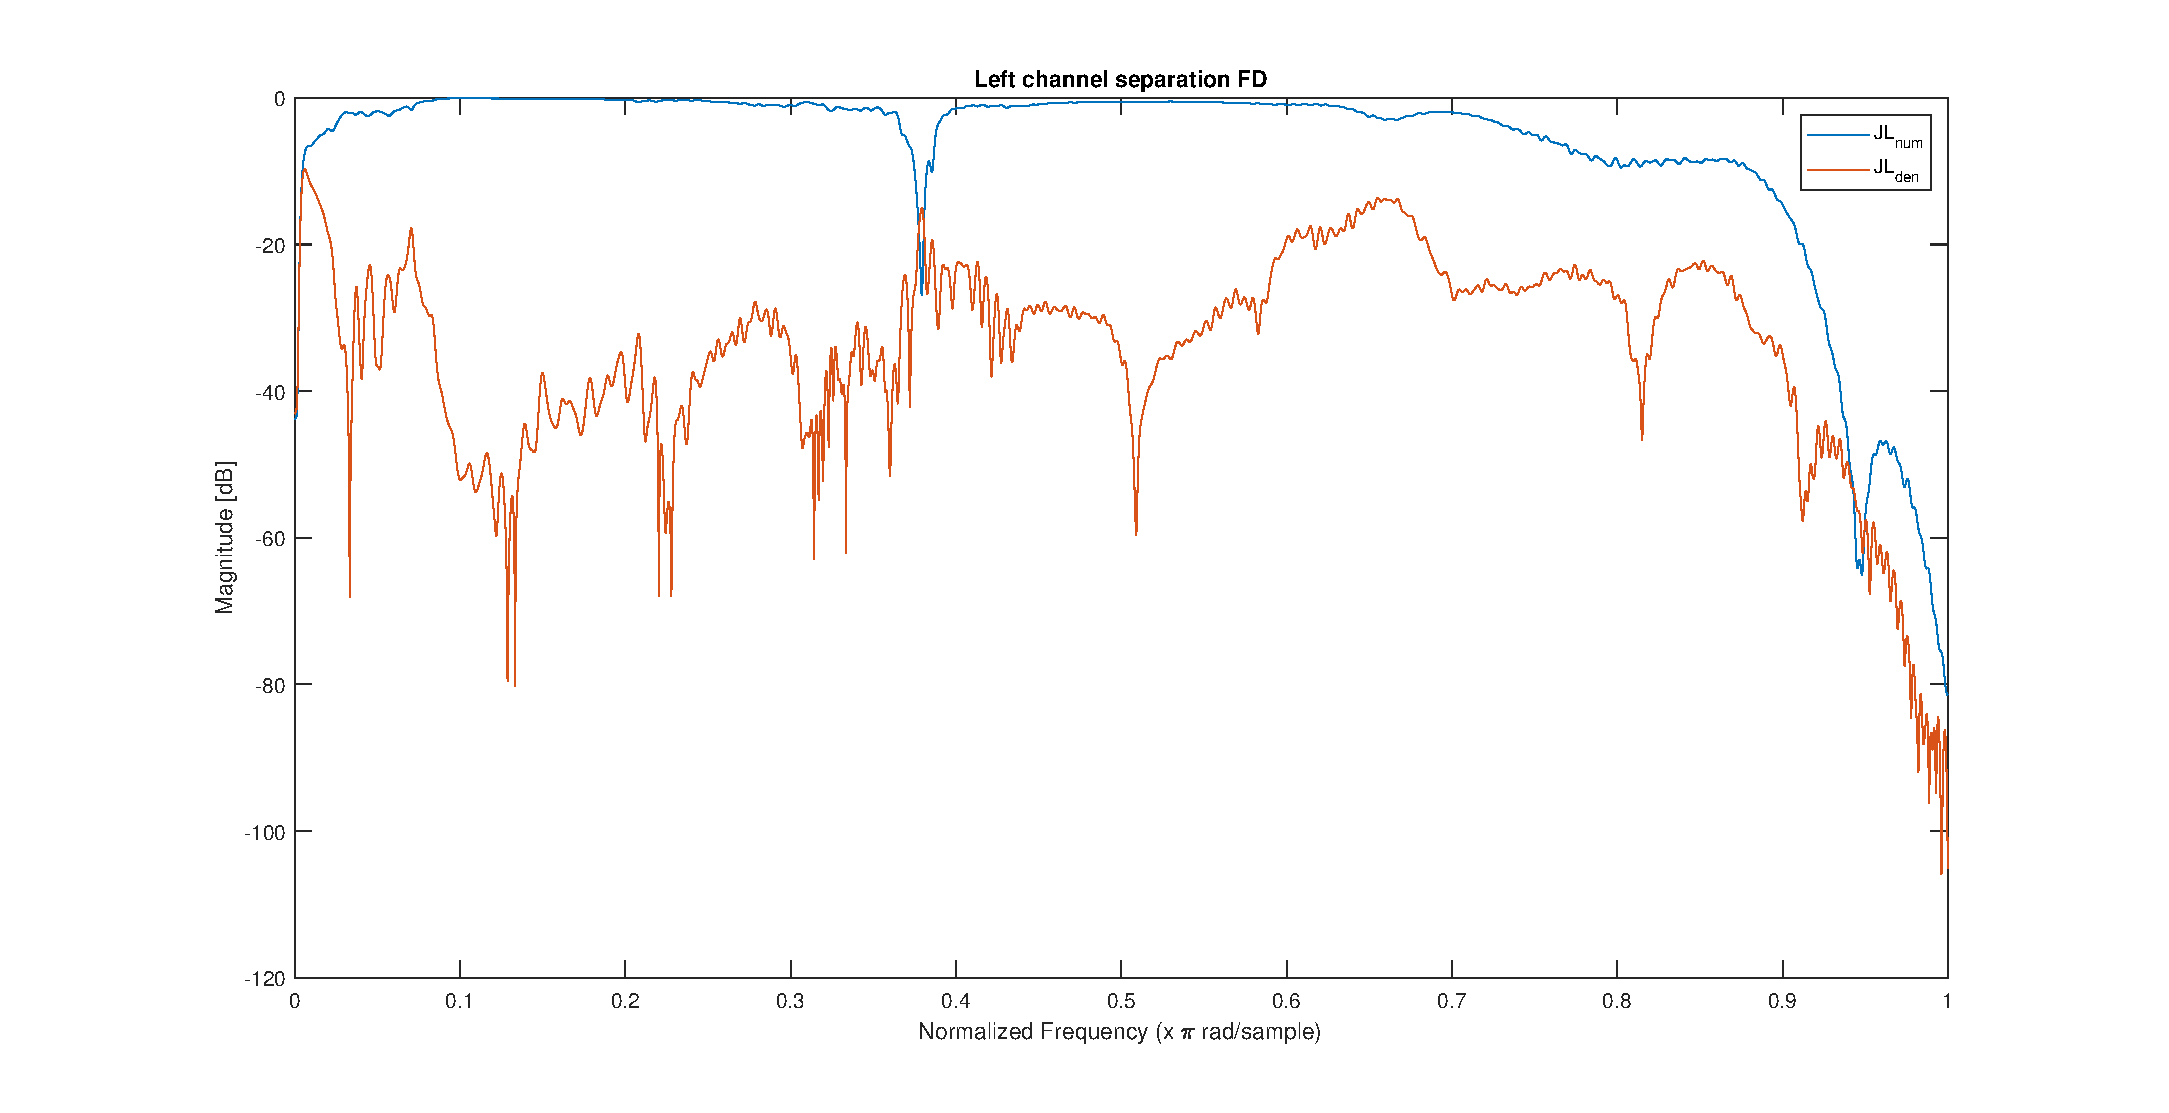
\includegraphics[width=1\textwidth]{Immagini/left_channel_separation_FD}
	\caption{}
	\label{left_channel_separation_FD}
\end{subfigure}
\hfill
\begin{subfigure}{.45\textwidth}
	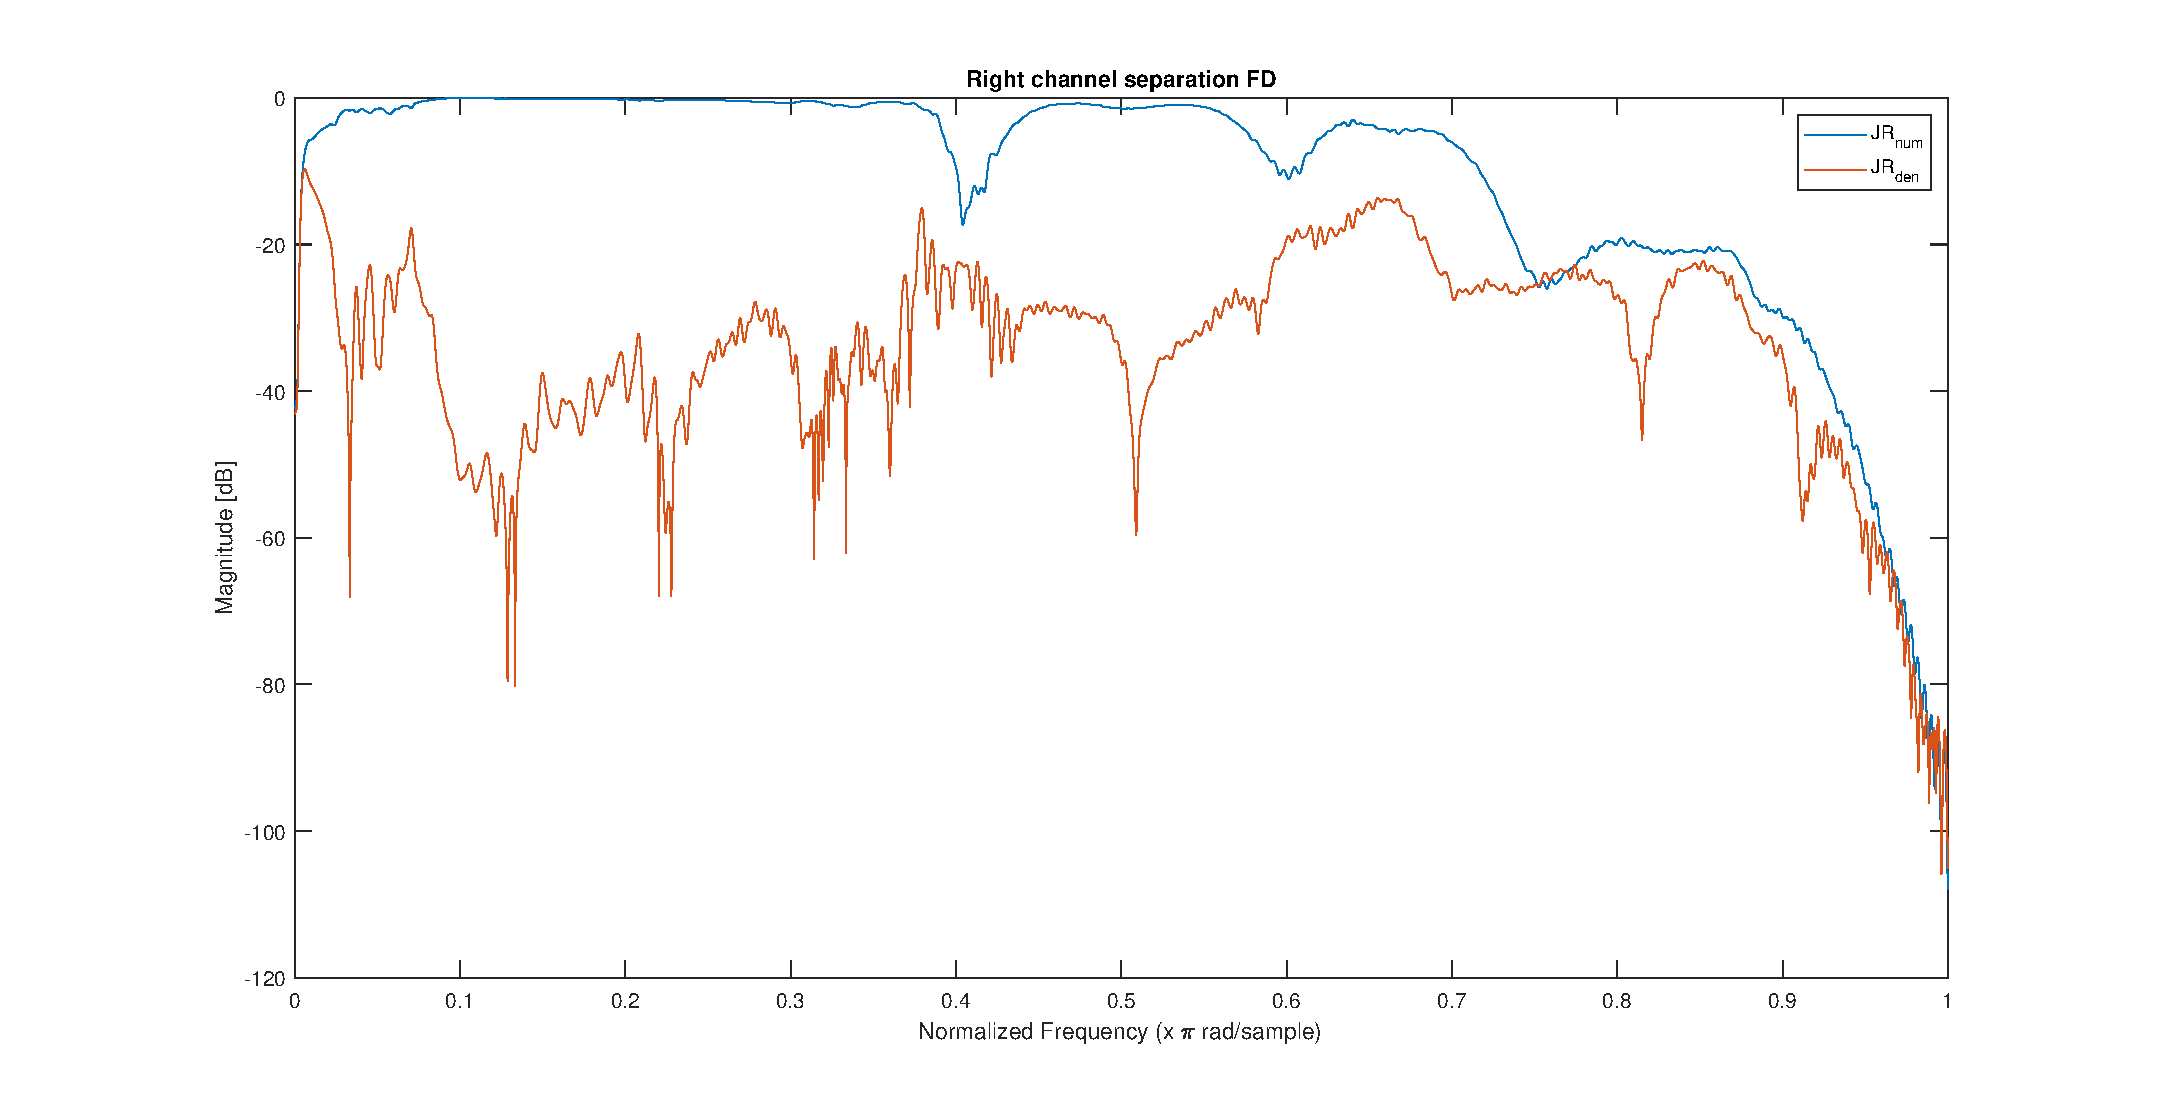
\includegraphics[width=1\textwidth]{Immagini/right_channel_separation_FD}
	\caption{}
	\label{right_channel_separation_FD}
\end{subfigure}
\vfill
\begin{subfigure}{.45\textwidth}
	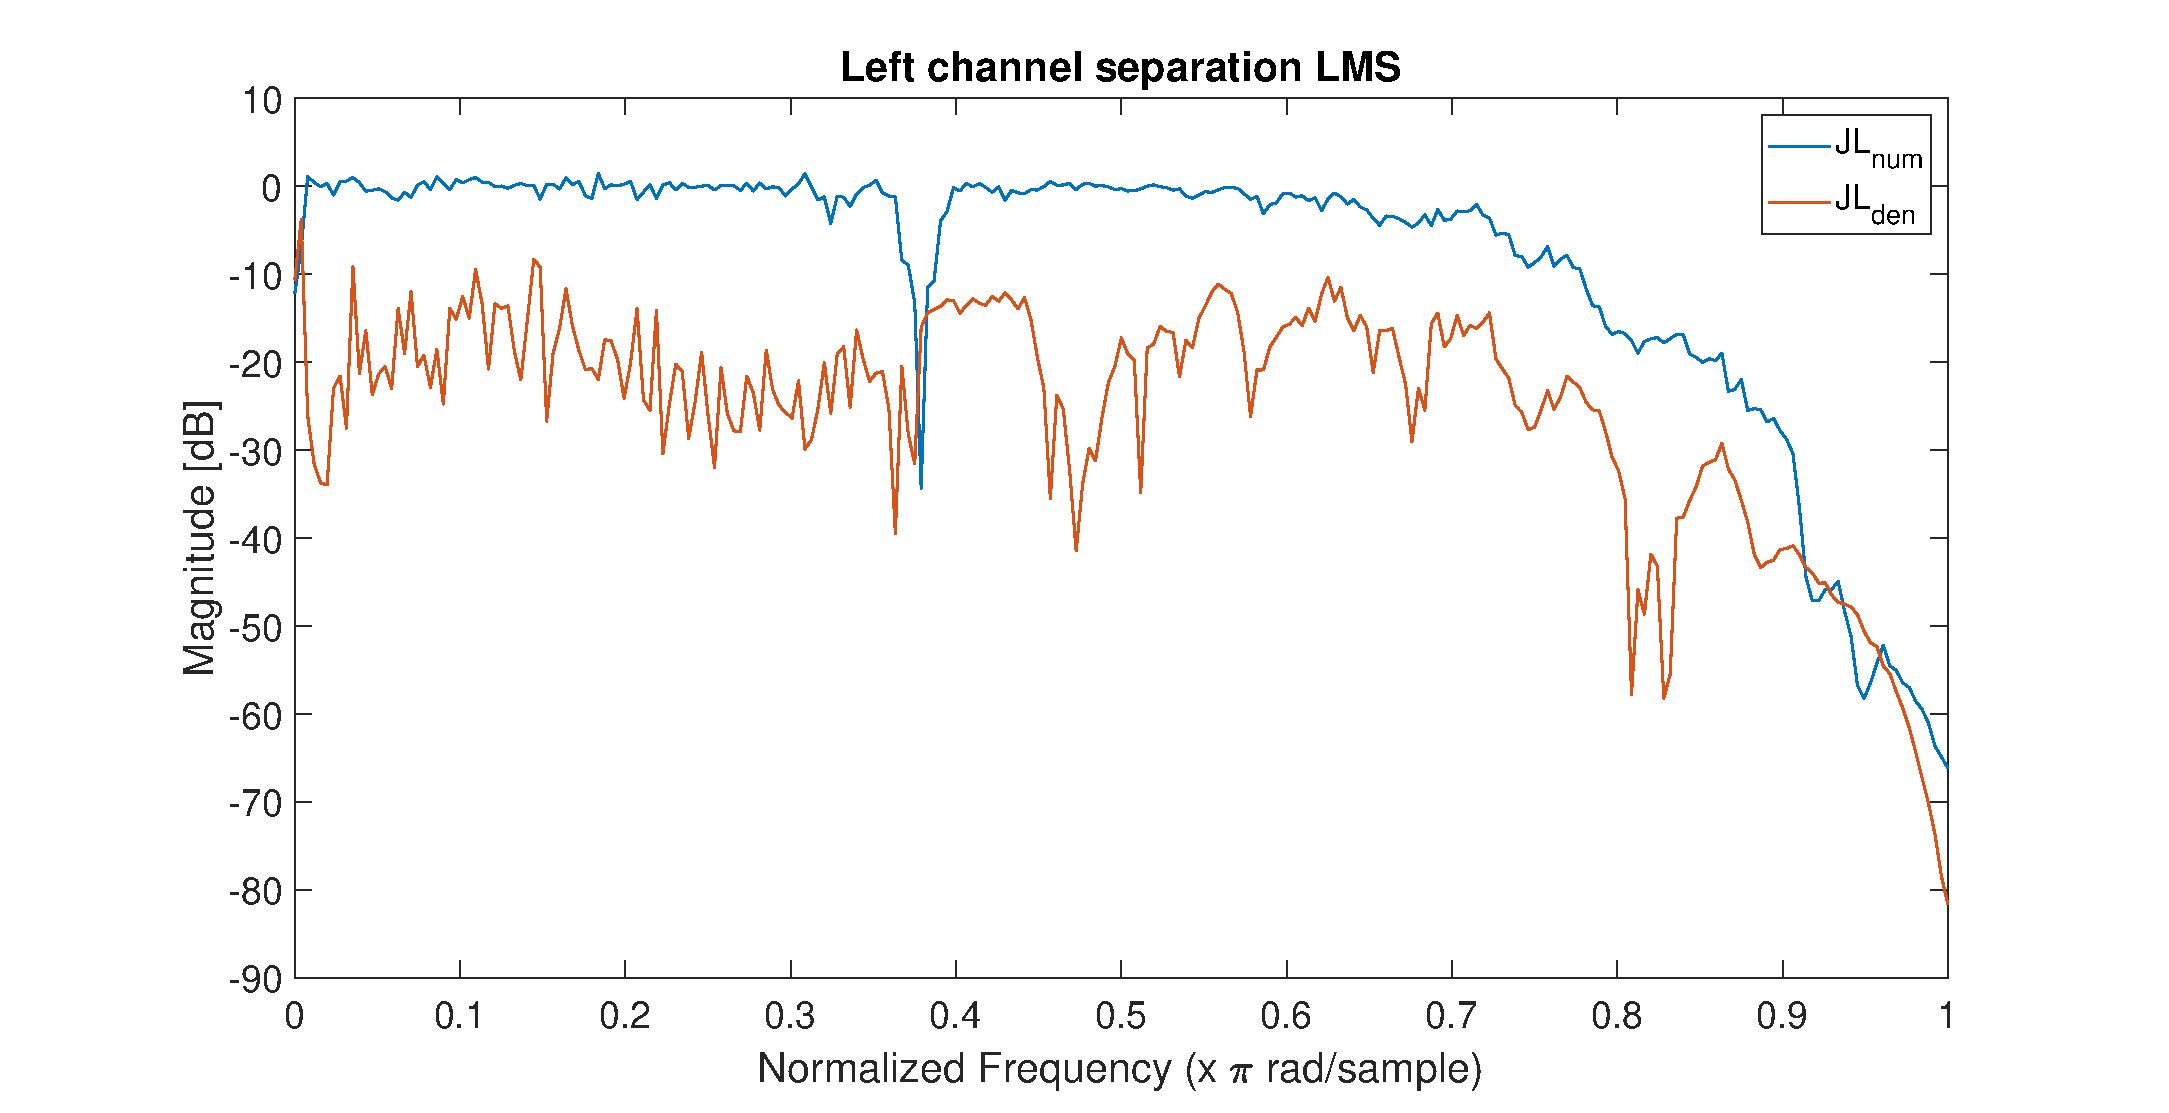
\includegraphics[width=1\textwidth]{Immagini/left_channel_separation_LMS}
	\caption{}
	\label{left_channel_separation_LMS}
\end{subfigure}
\hfill
\begin{subfigure}{.45\textwidth}
	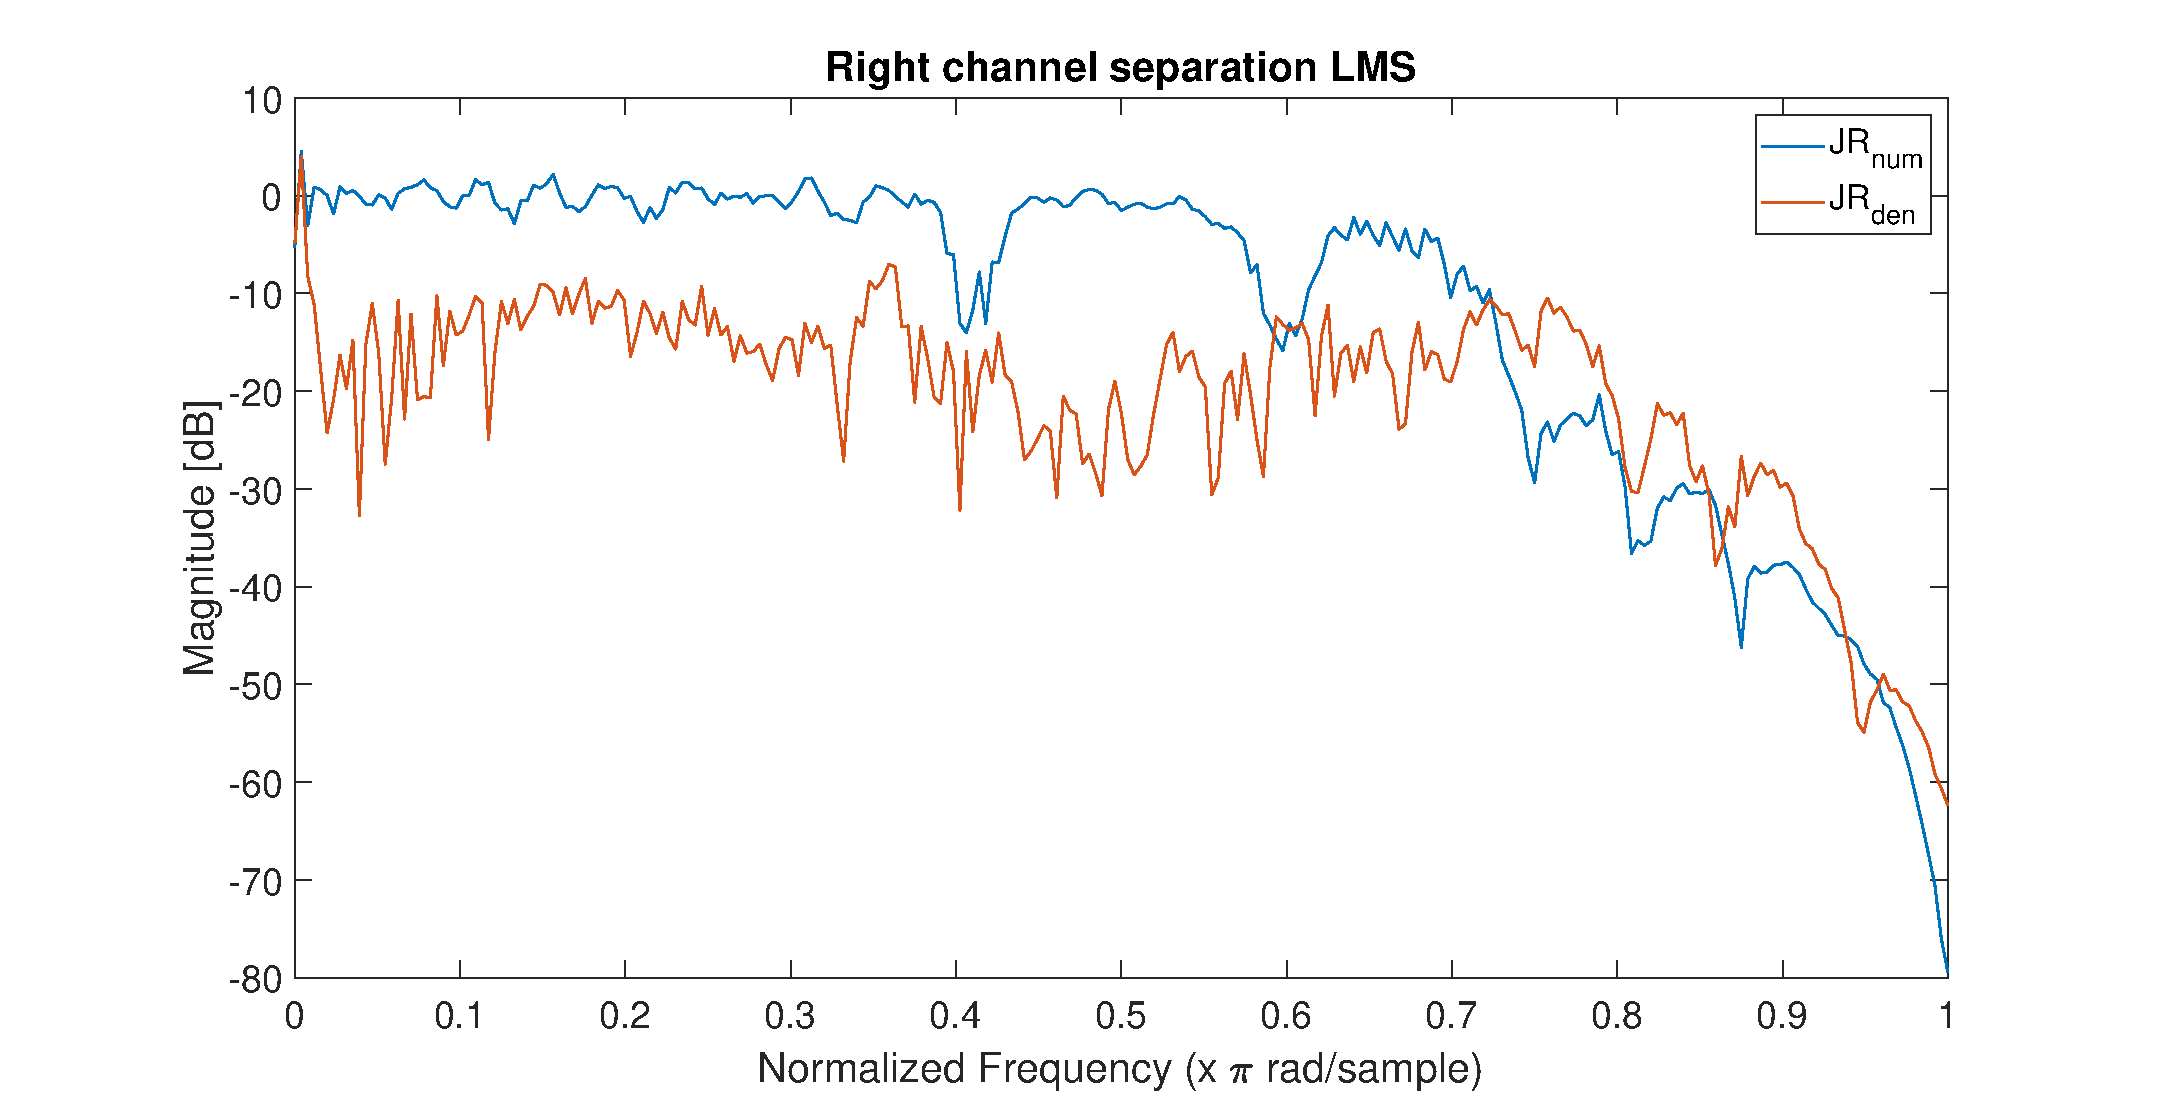
\includegraphics[width=1\textwidth]{Immagini/right_channel_separation_LMS}
	\caption{}
	\label{right_channel_separation_LMS}
\end{subfigure}
\caption{Confronto del numeratore e del denominatore di (a) $J_L$ e (b) $J_R$ per FD con $\beta = 0.3$, (c) $J_L$ e (d) $J_R$ per LMS con $\mu = 10^{-3}$.}
\label{fig:channel_separation_LMS_FD}
\end{figure}
\end{frame}

\begin{frame}
\begin{figure}[h]
	\begin{subfigure}{.45\textwidth}
		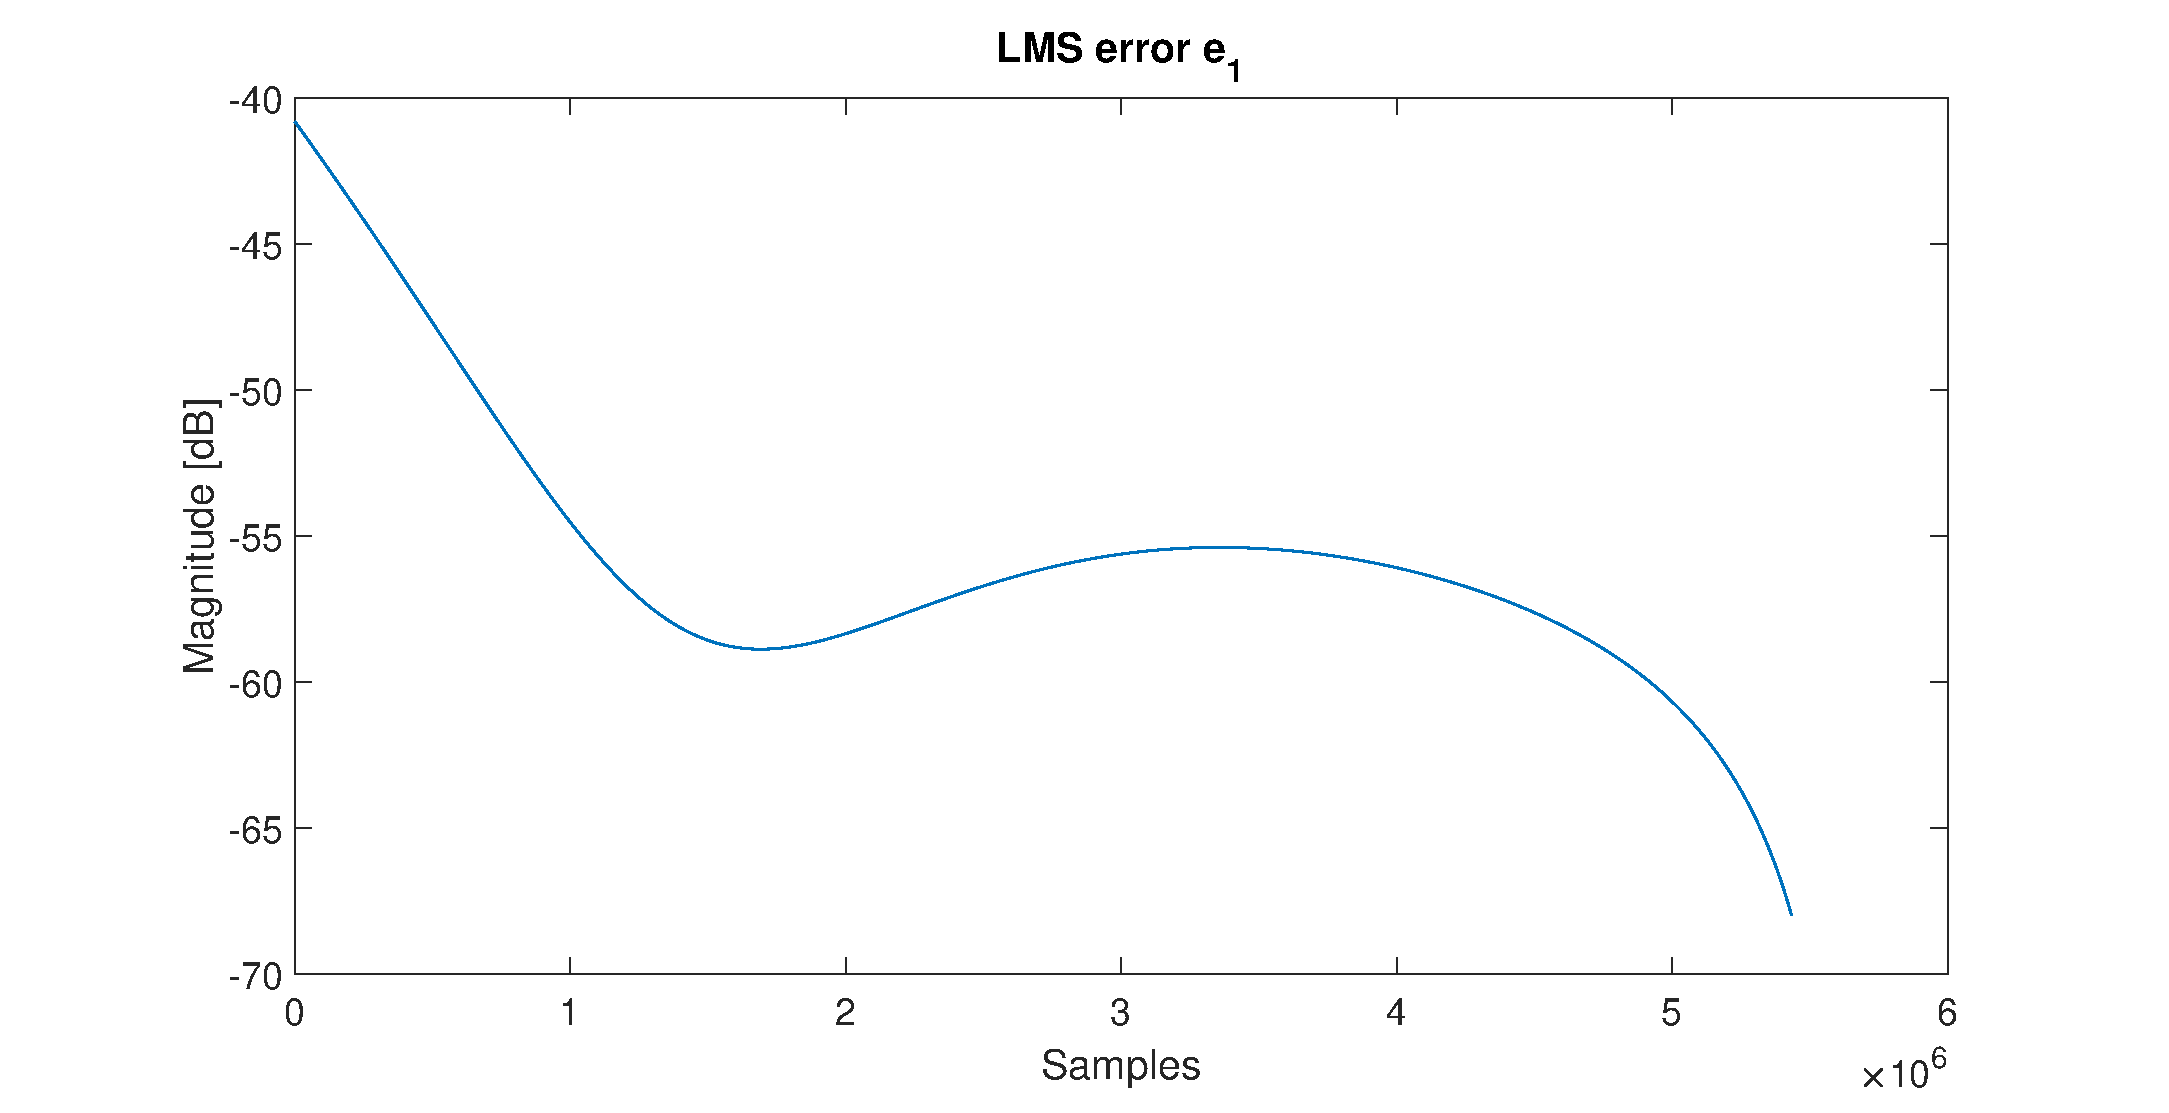
\includegraphics[width=1\textwidth]{Immagini/mse_e1}
		\caption{}
		\label{mse_e1}
	\end{subfigure}
	\vfill
	\begin{subfigure}{.45\textwidth}
		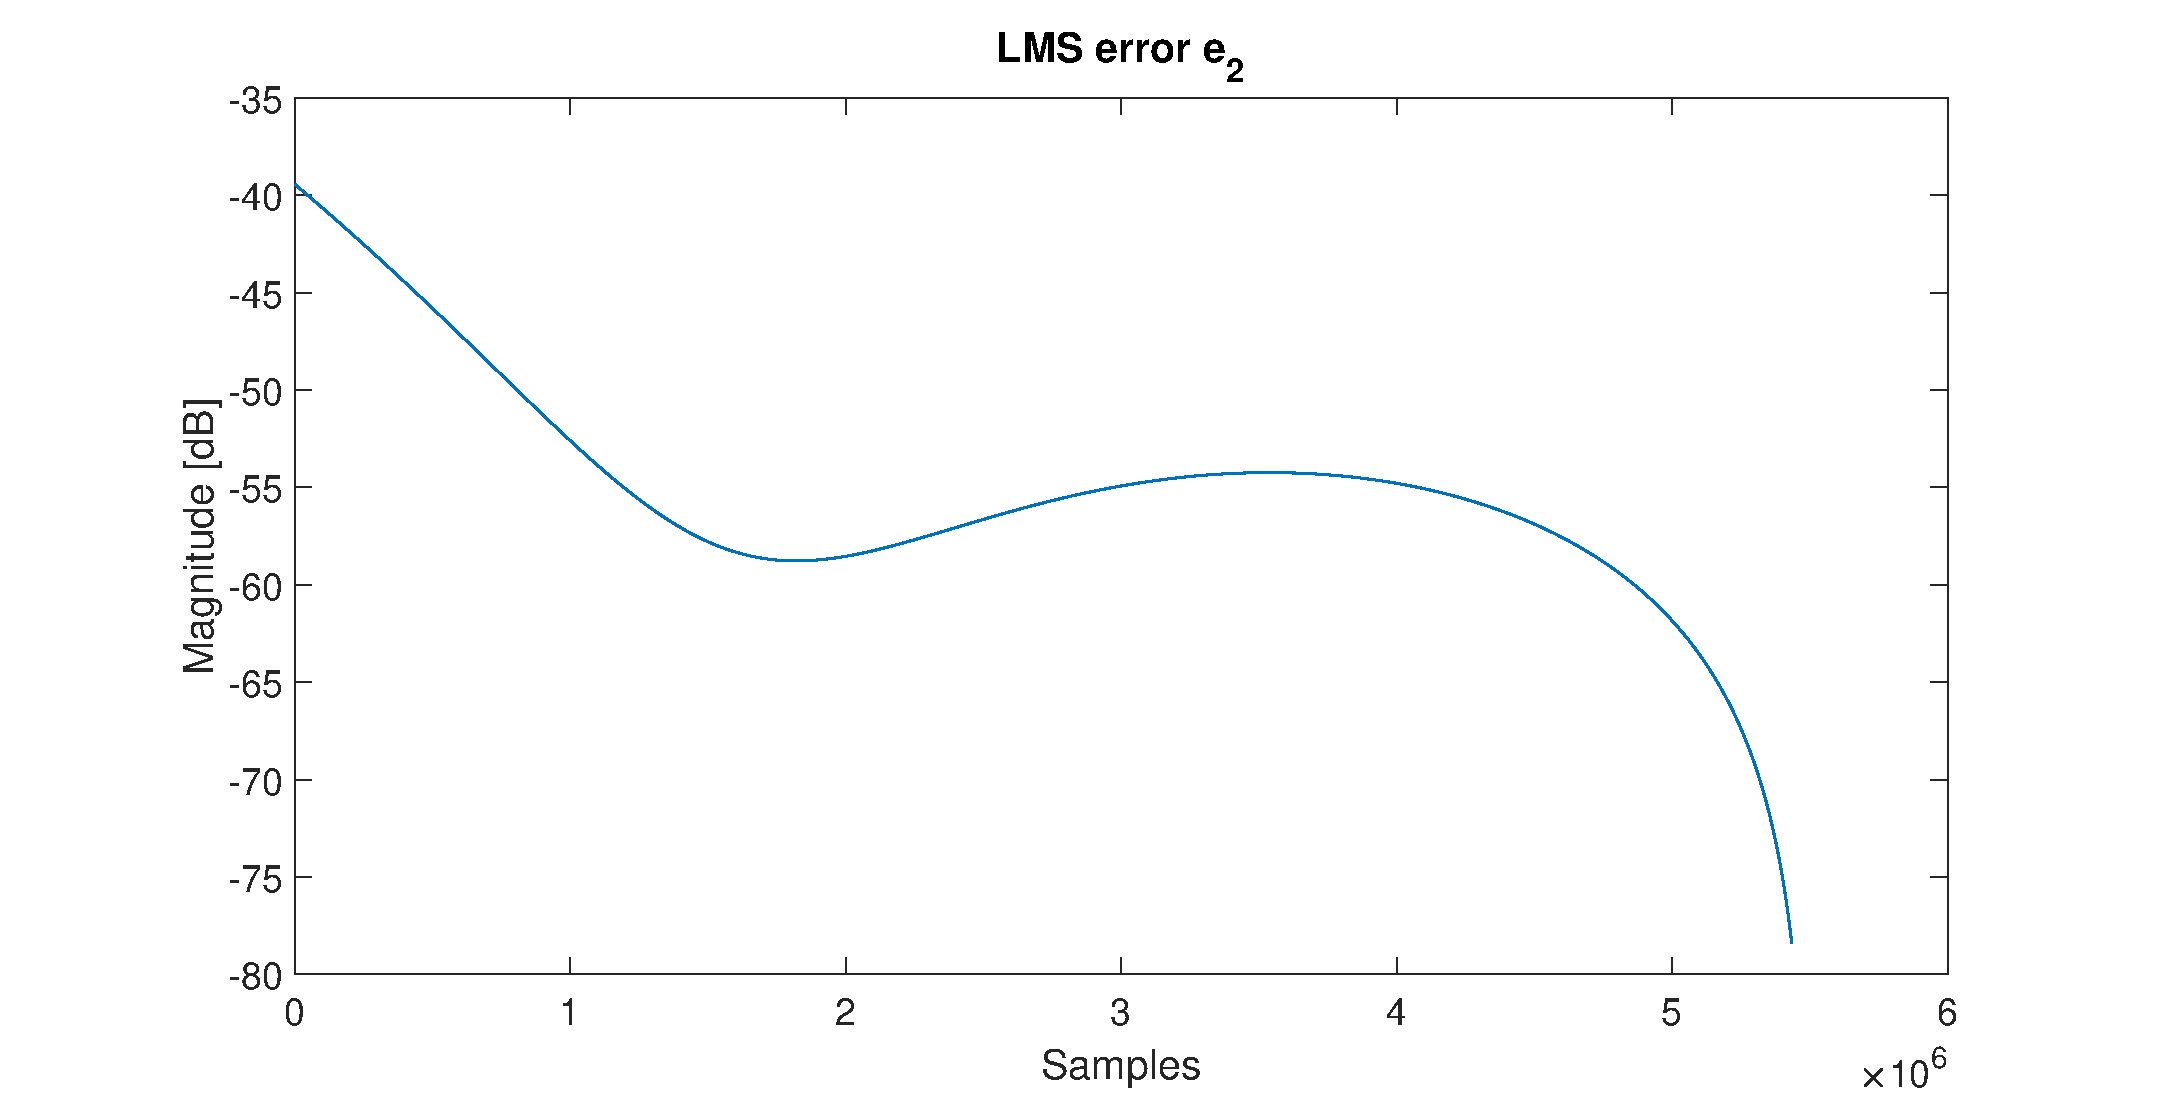
\includegraphics[width=1\textwidth]{Immagini/mse_e2}
		\caption{}
		\label{mse_e2}
	\end{subfigure}
	\caption{Confronto dell'MSE del canale (a) sinistro e (b) destro dell'algoritmo LMS.}
	\label{fig:mse_LMS}
\end{figure}
\end{frame}

\begin{frame}
\begin{figure}[h]
	\centering
	\begin{subfigure}{.45\textwidth}
		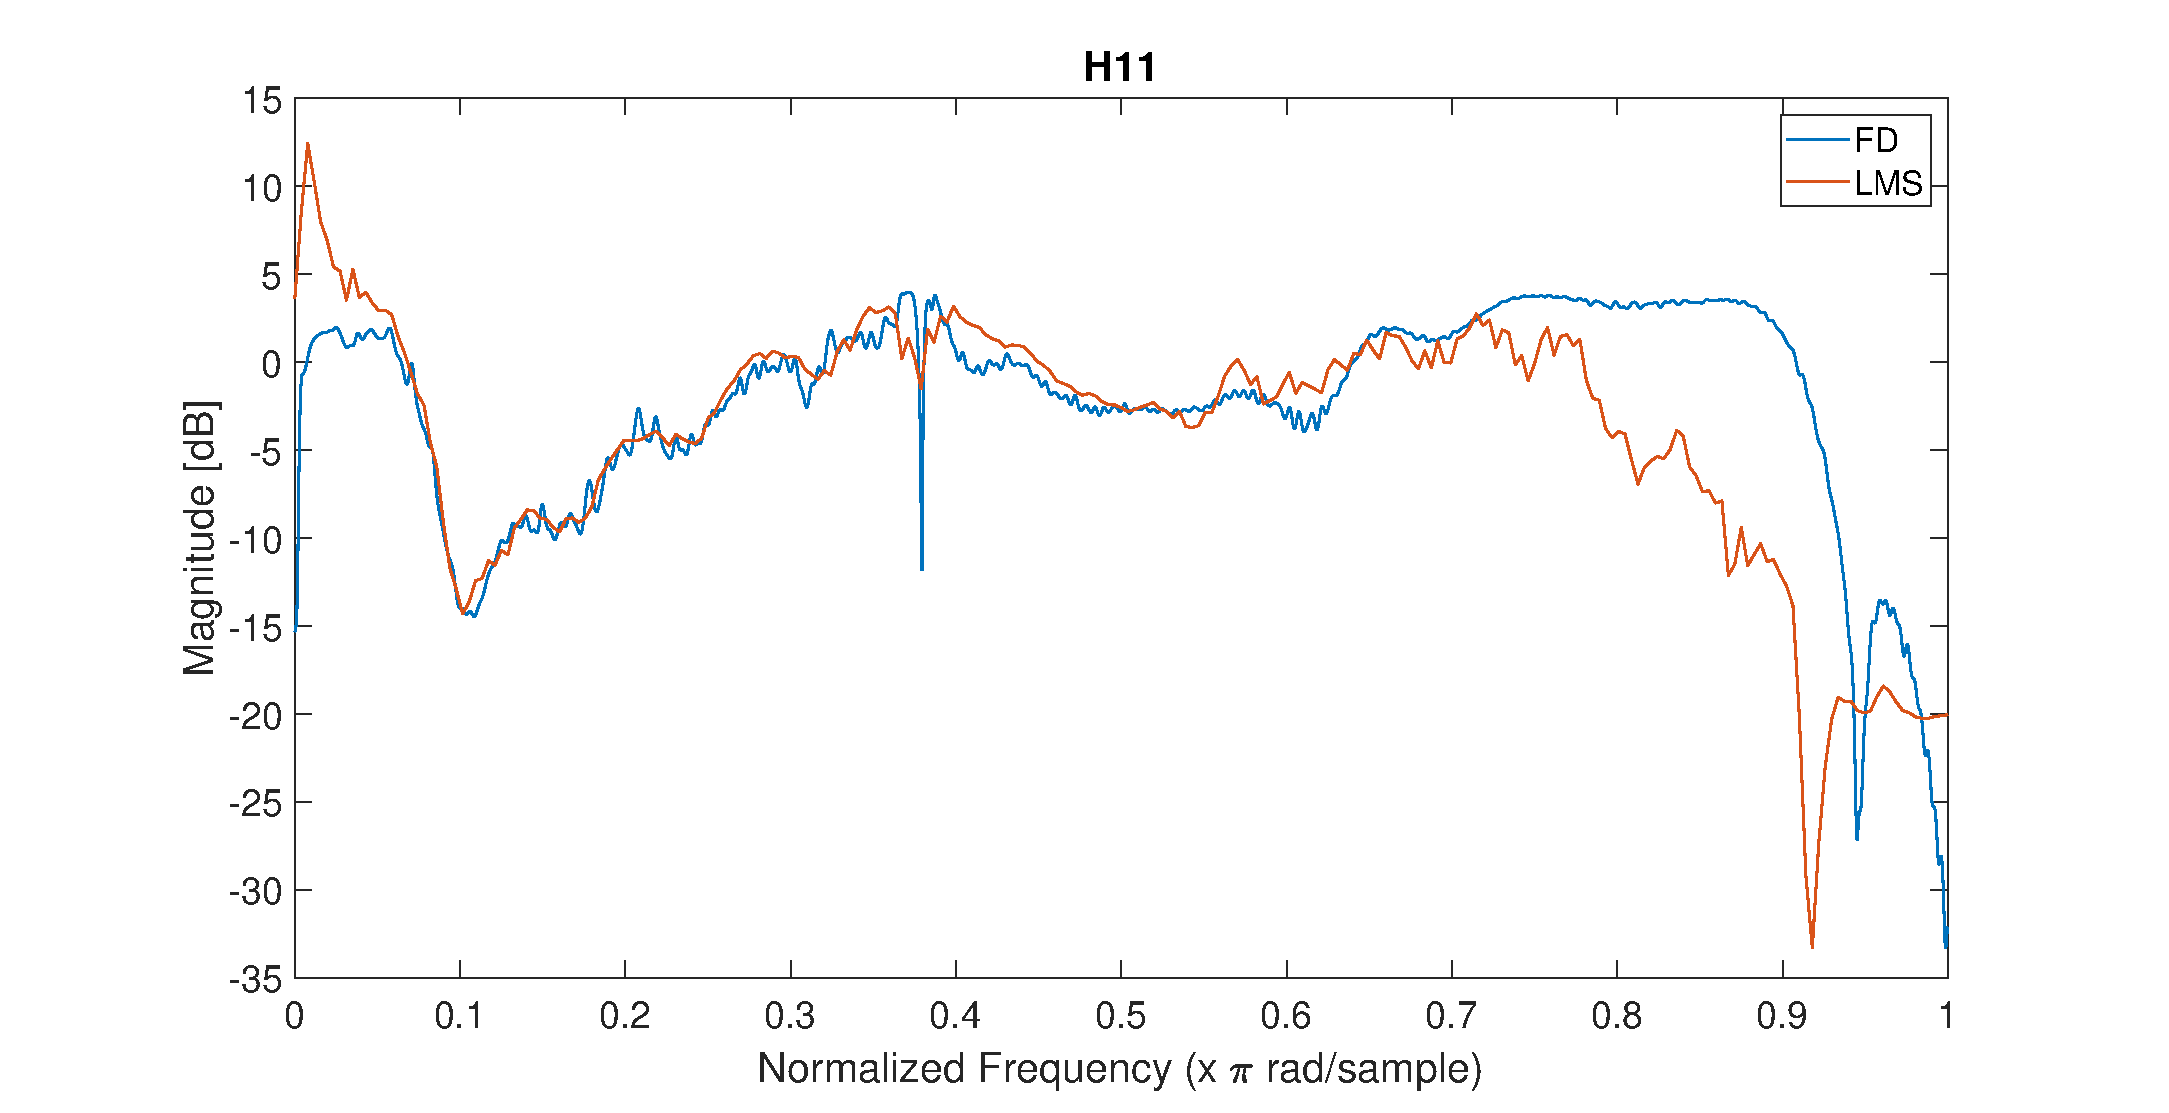
\includegraphics[width=1\textwidth]{Immagini/H11_FD_LMS}
		\caption{}
		\label{fig:Confronto_H11_LMS_FD}
	\end{subfigure}
	\hfill
	\begin{subfigure}{.45\textwidth}
		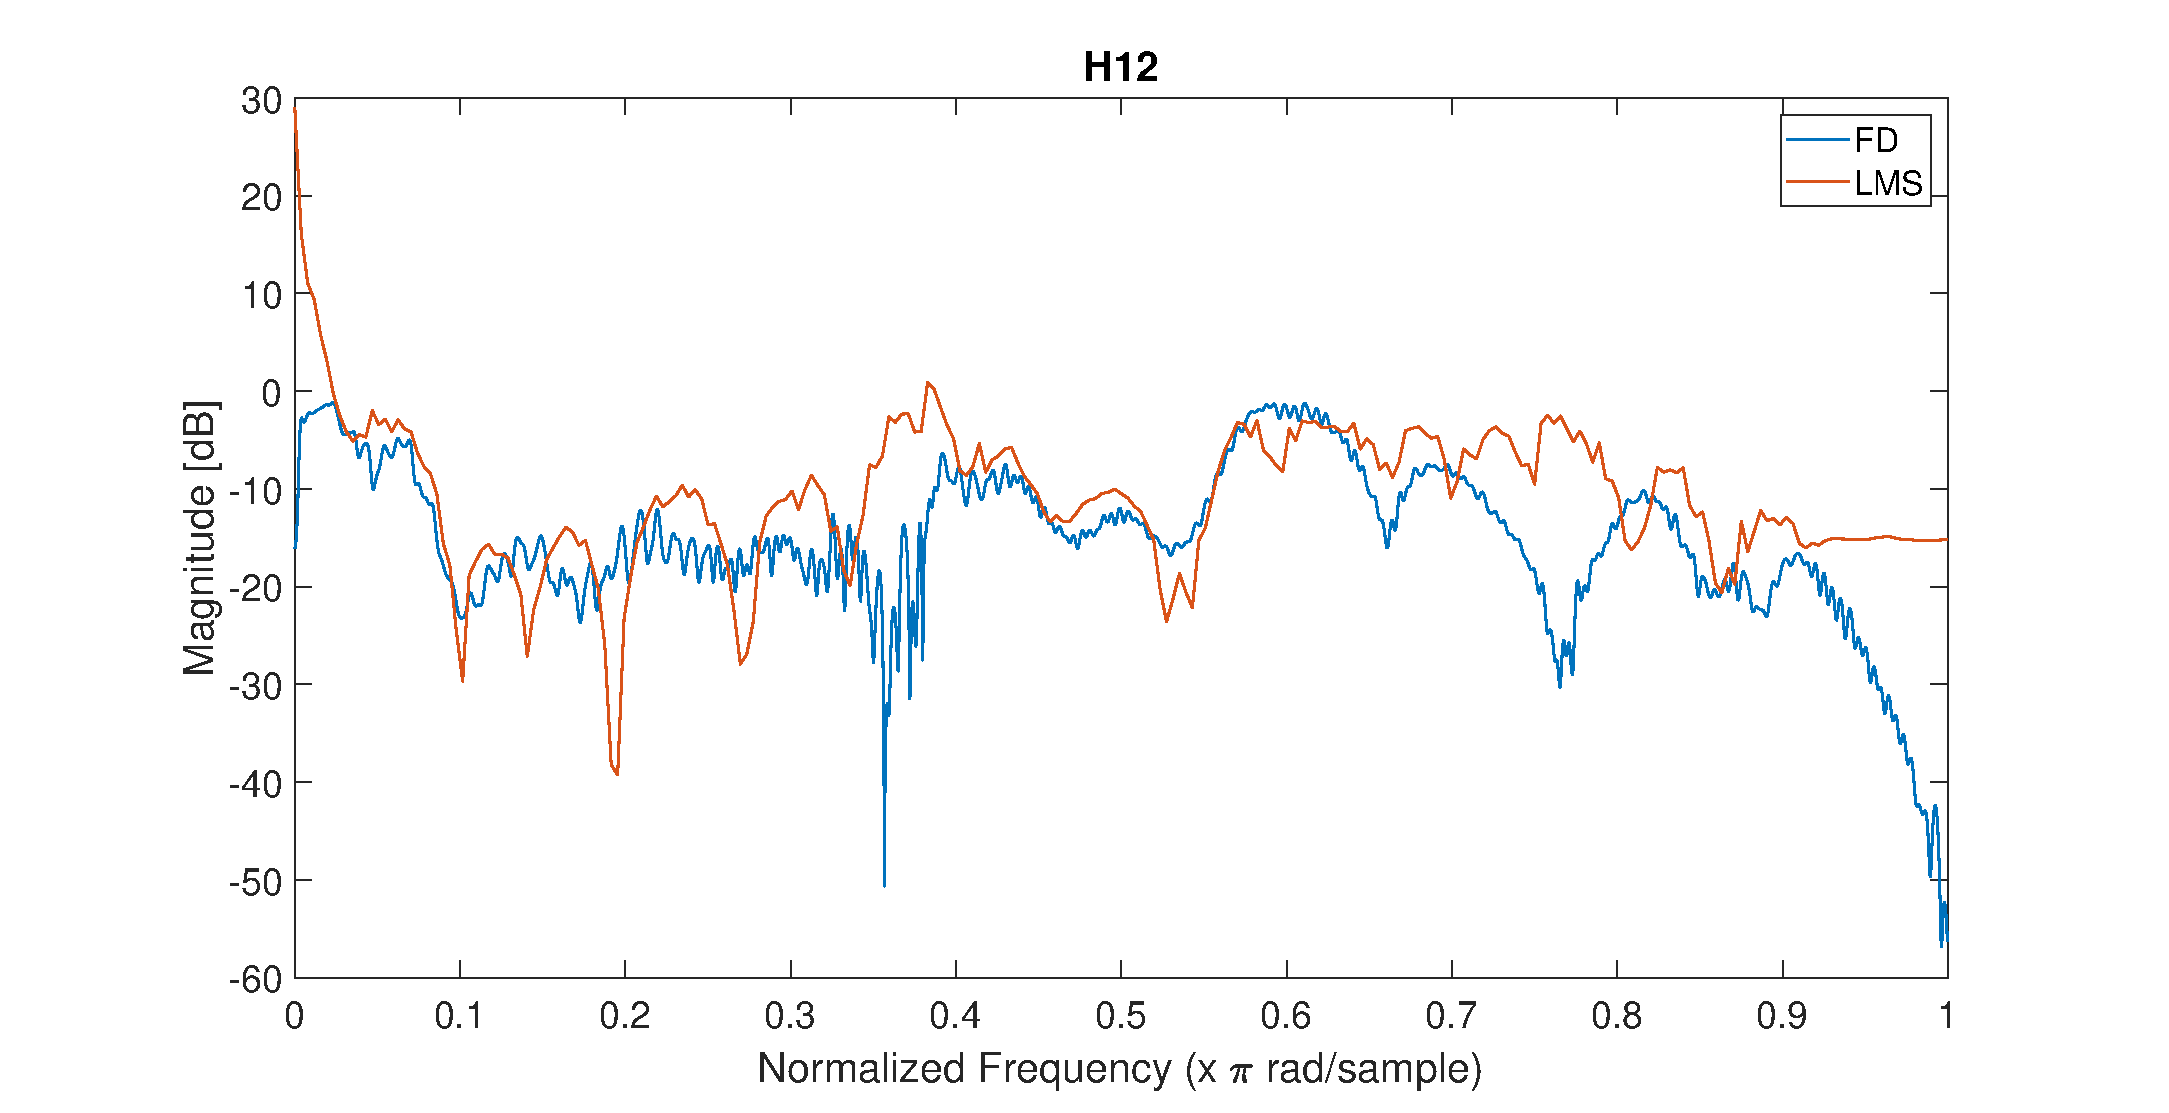
\includegraphics[width=1\textwidth]{Immagini/H12_FD_LMS}
		\caption{}
		\label{fig:Confronto_H12_LMS_FD}
	\end{subfigure}
	\vfill
	\begin{subfigure}{.45\textwidth}
		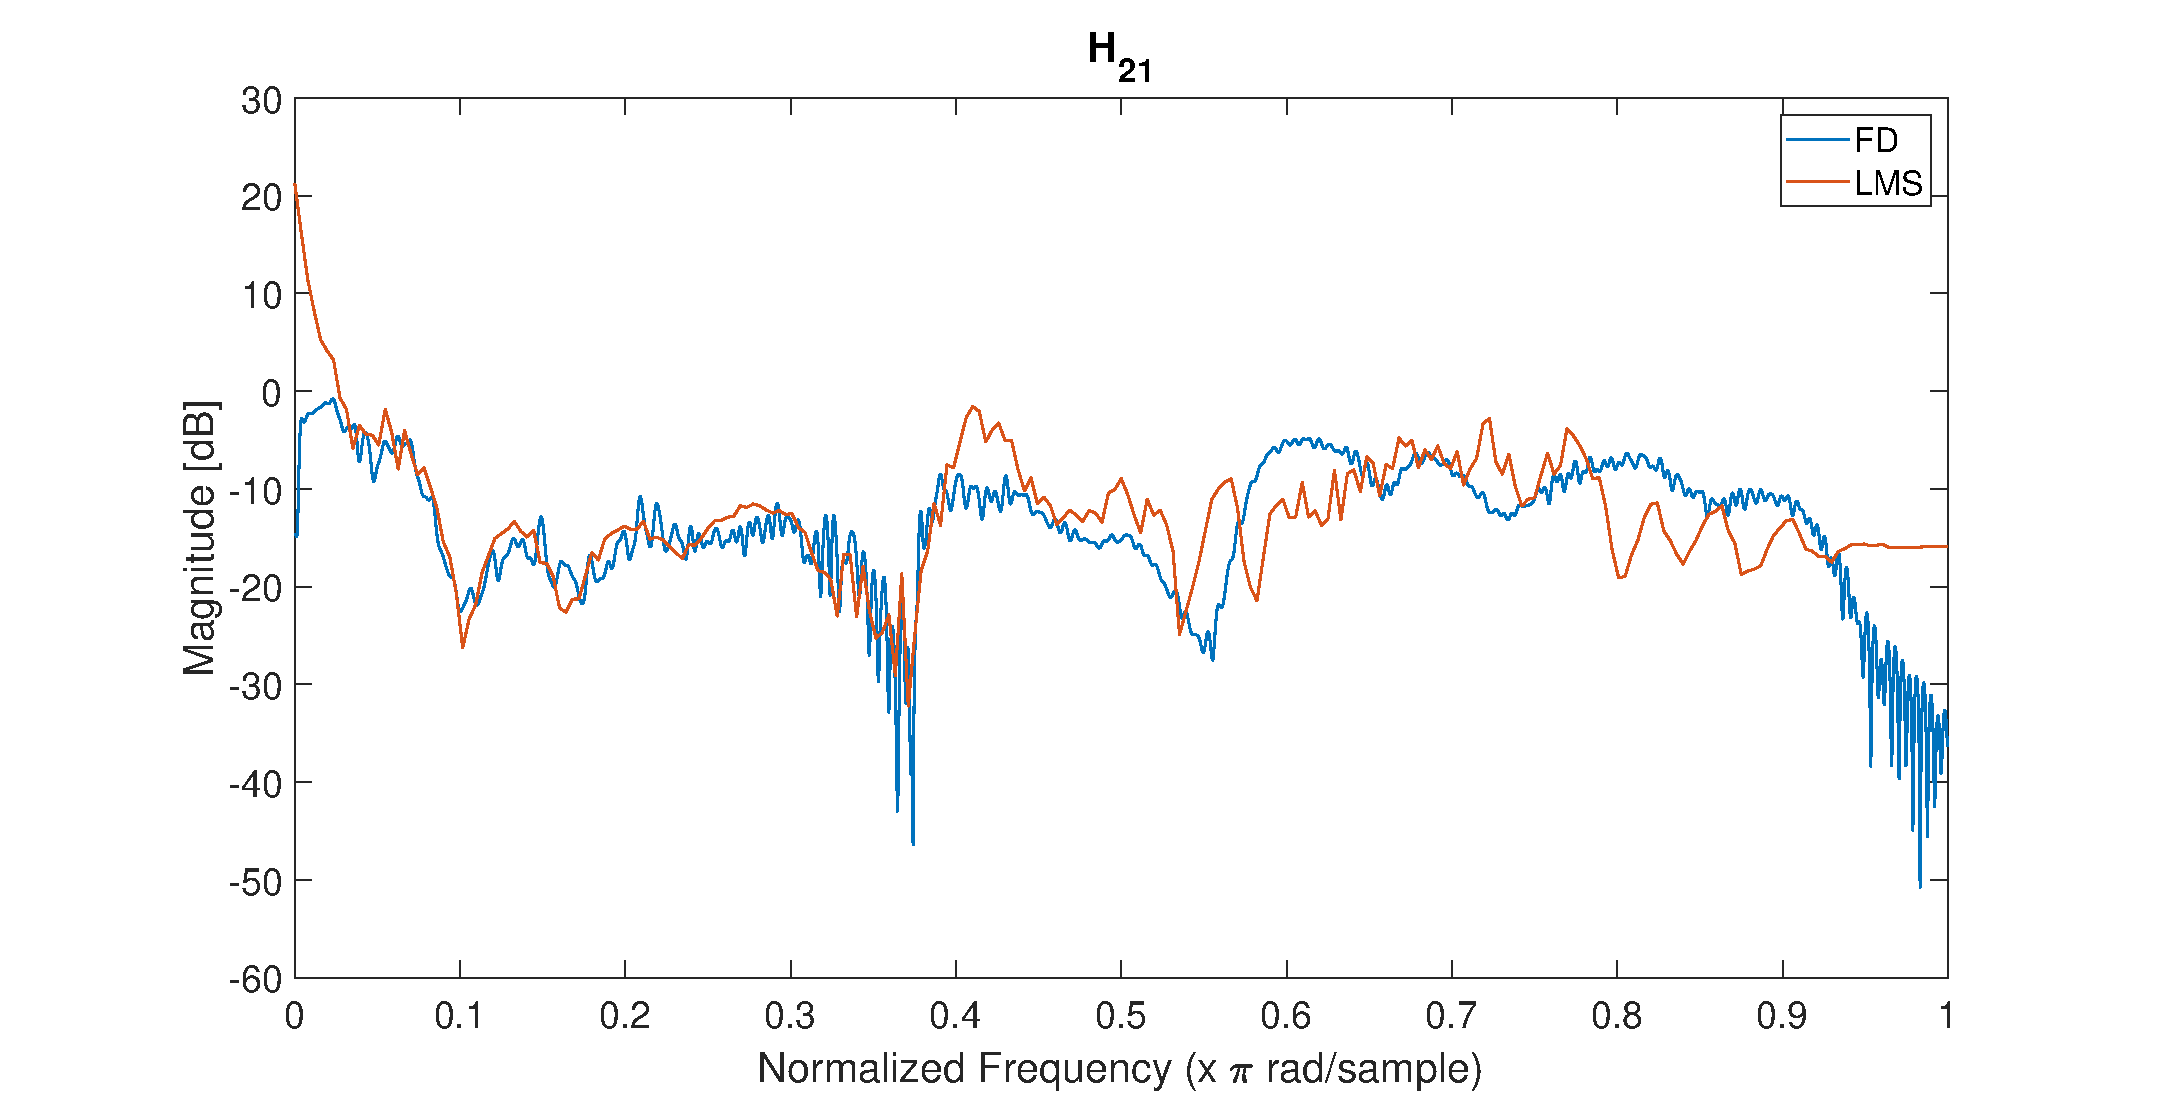
\includegraphics[width=1\textwidth]{Immagini/H21_FD_LMS}
		\caption{}
		\label{fig:Confronto_H21_LMS_FD}
	\end{subfigure}
	\hfill
	\begin{subfigure}{.45\textwidth}
		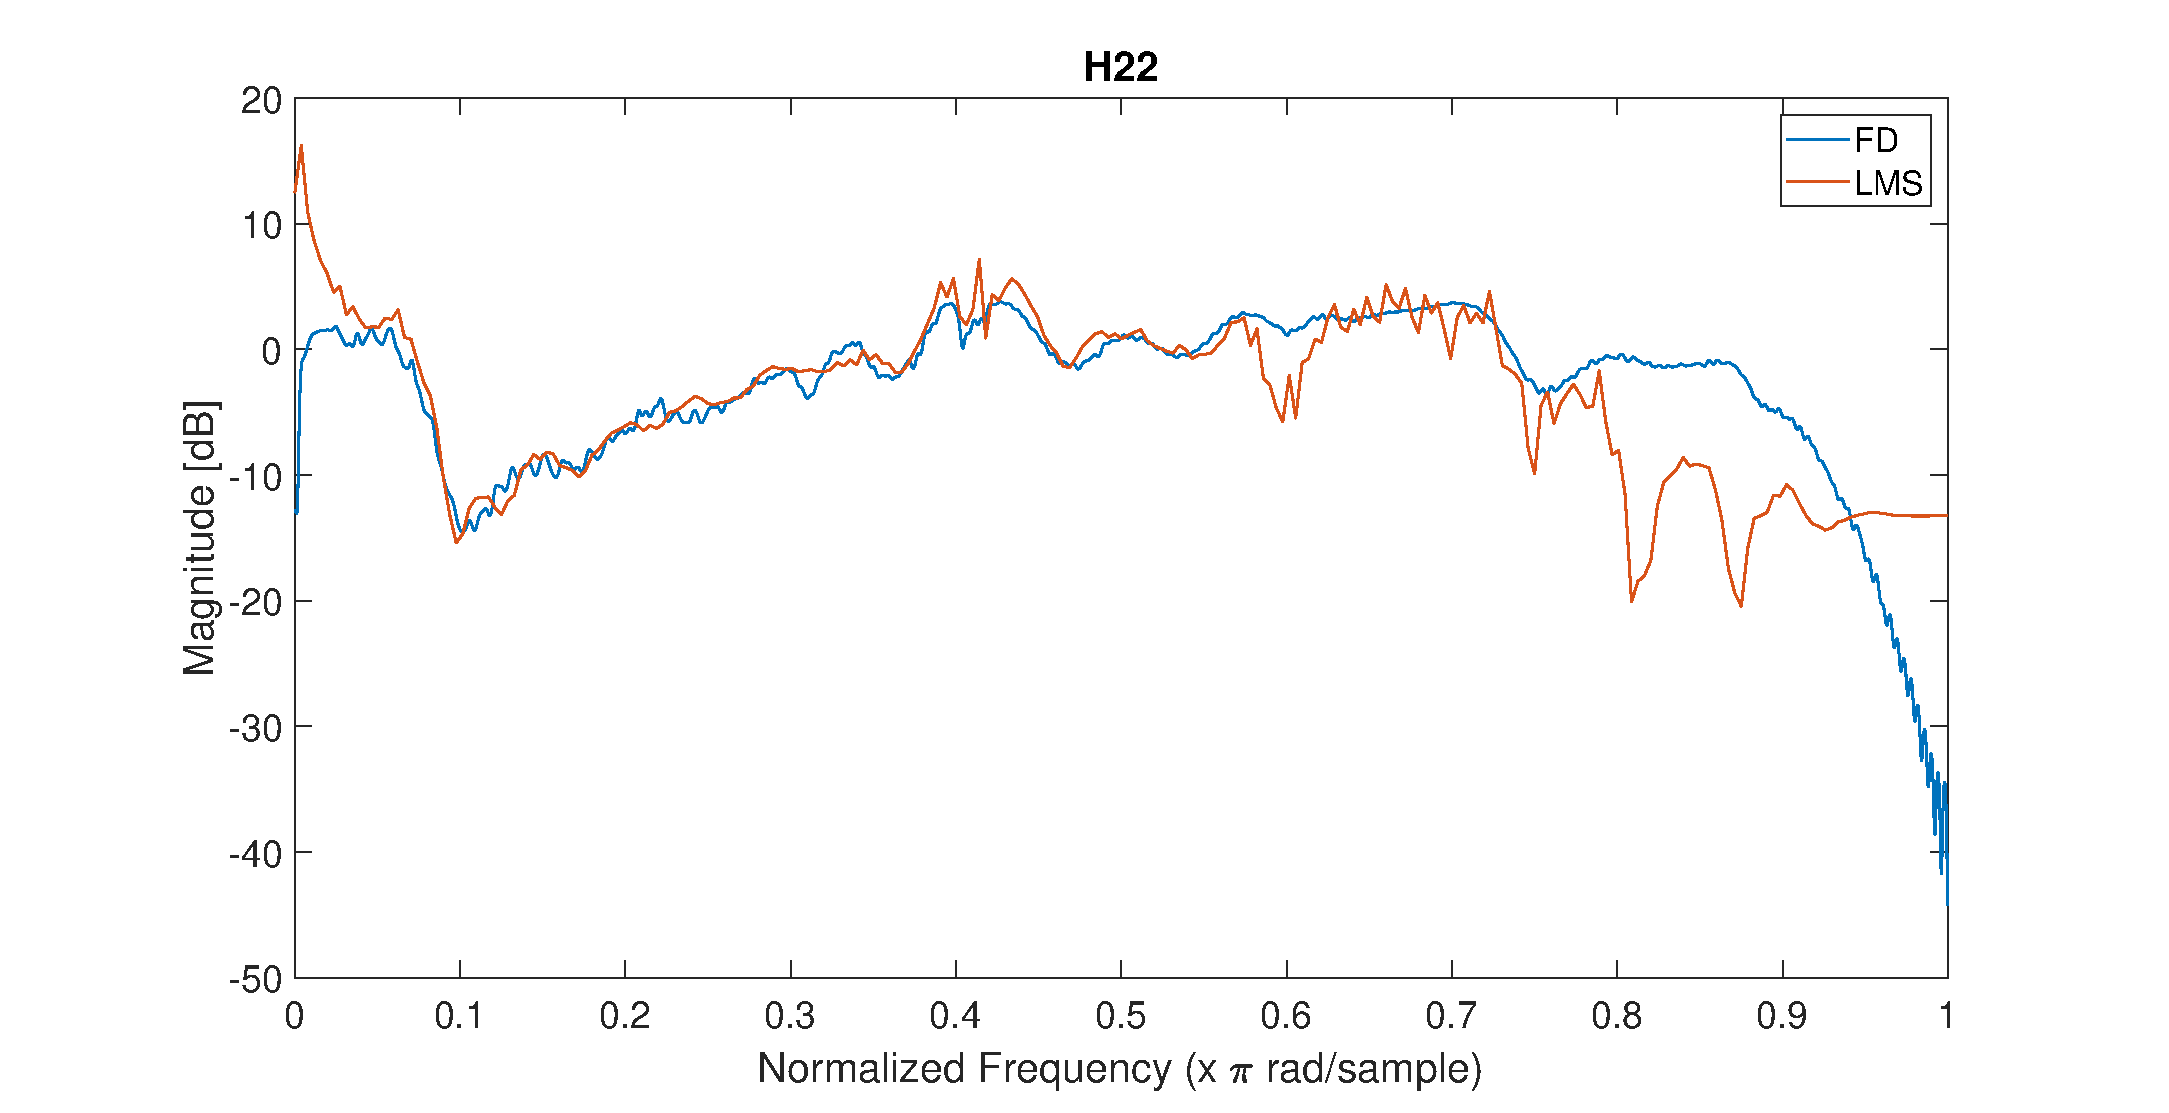
\includegraphics[width=1\textwidth]{Immagini/H22_FD_LMS}
		\caption{}
		\label{fig:Confronto_H22_LMS_FD}
	\end{subfigure}
	\caption{Confronto dei filtri di cancellazione del crosstalk (a) $H_{11}$, (b) $H_{12}$, (c) $H_{21}$, (d) $H_{22}$ di LMS e Fast Deconvolution.}
	\label{fig:confronto_H_LMS_FD}
\end{figure}
\end{frame}

\begin{frame}
\begin{figure}[h]
	\centering
	\begin{subfigure}{.45\textwidth}
		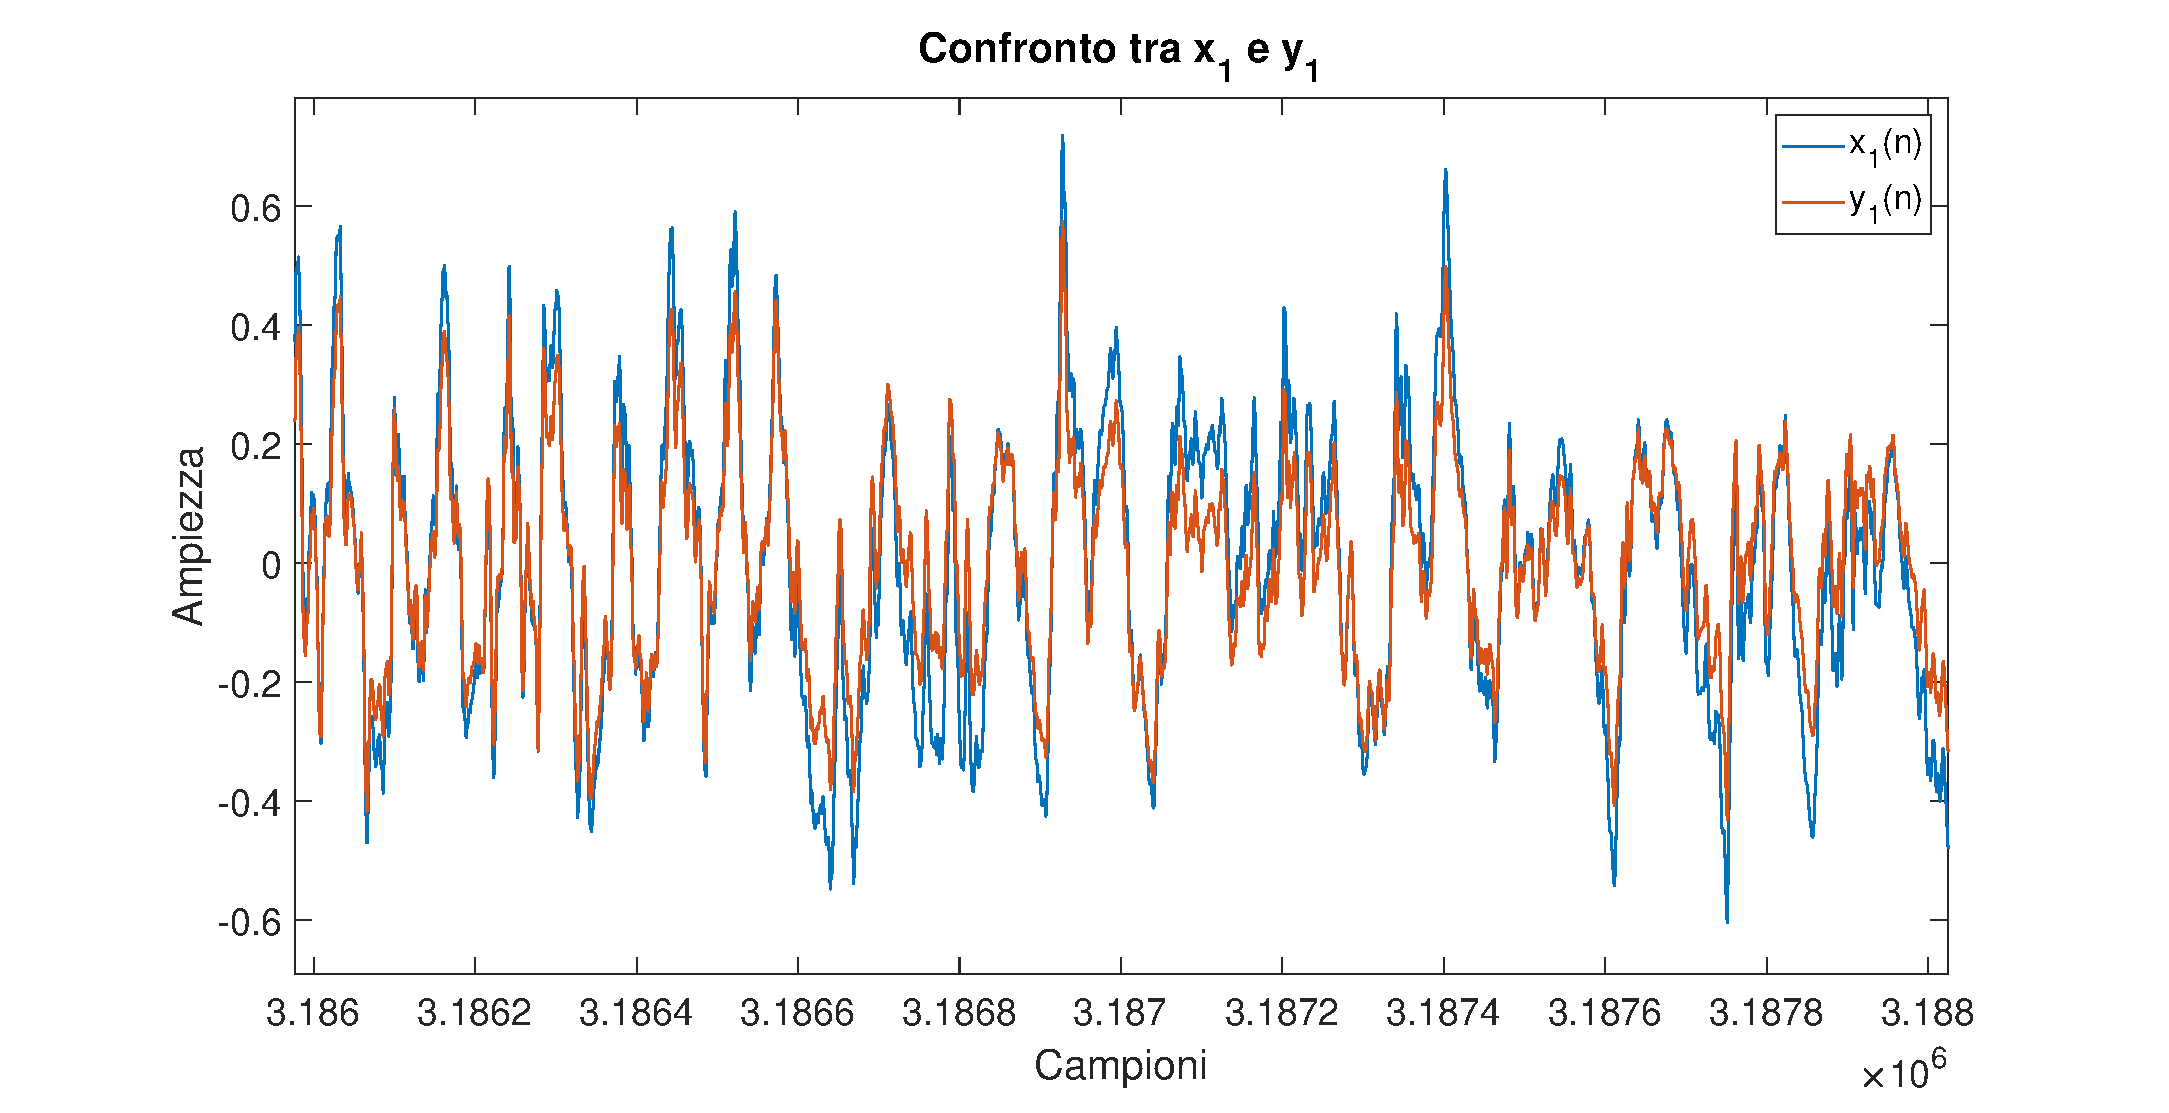
\includegraphics[width=1\textwidth]{Immagini/x1_y1_FD}
		\caption{}
		\label{fig:x1_y1_FD}
	\end{subfigure}
	\hfill
	\begin{subfigure}{.45\textwidth}
		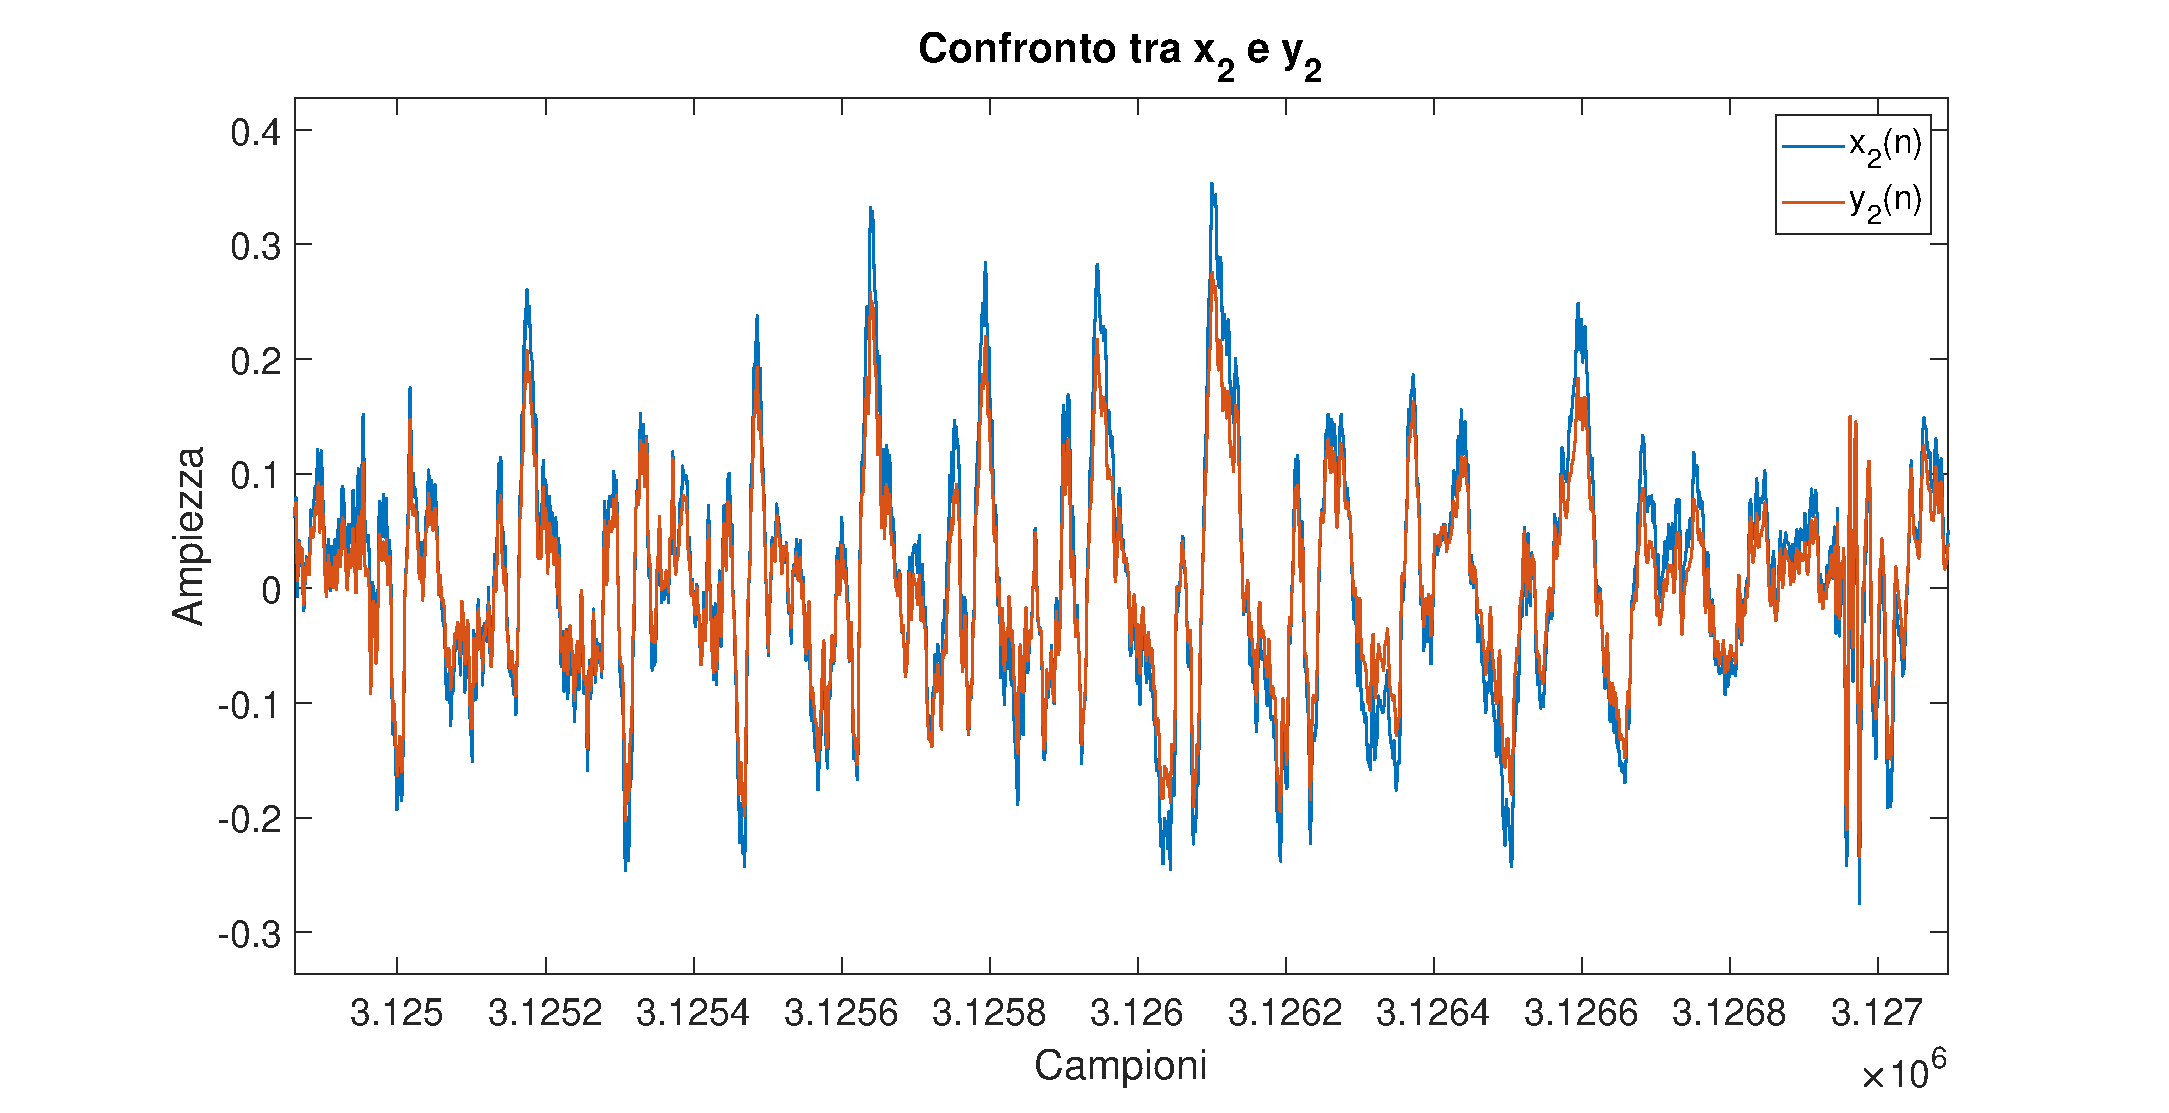
\includegraphics[width=1\textwidth]{Immagini/x2_y2_FD}
		\caption{}
		\label{fig:x2_y2_FD}
	\end{subfigure}
	\vfill
	\begin{subfigure}{.45\textwidth}
		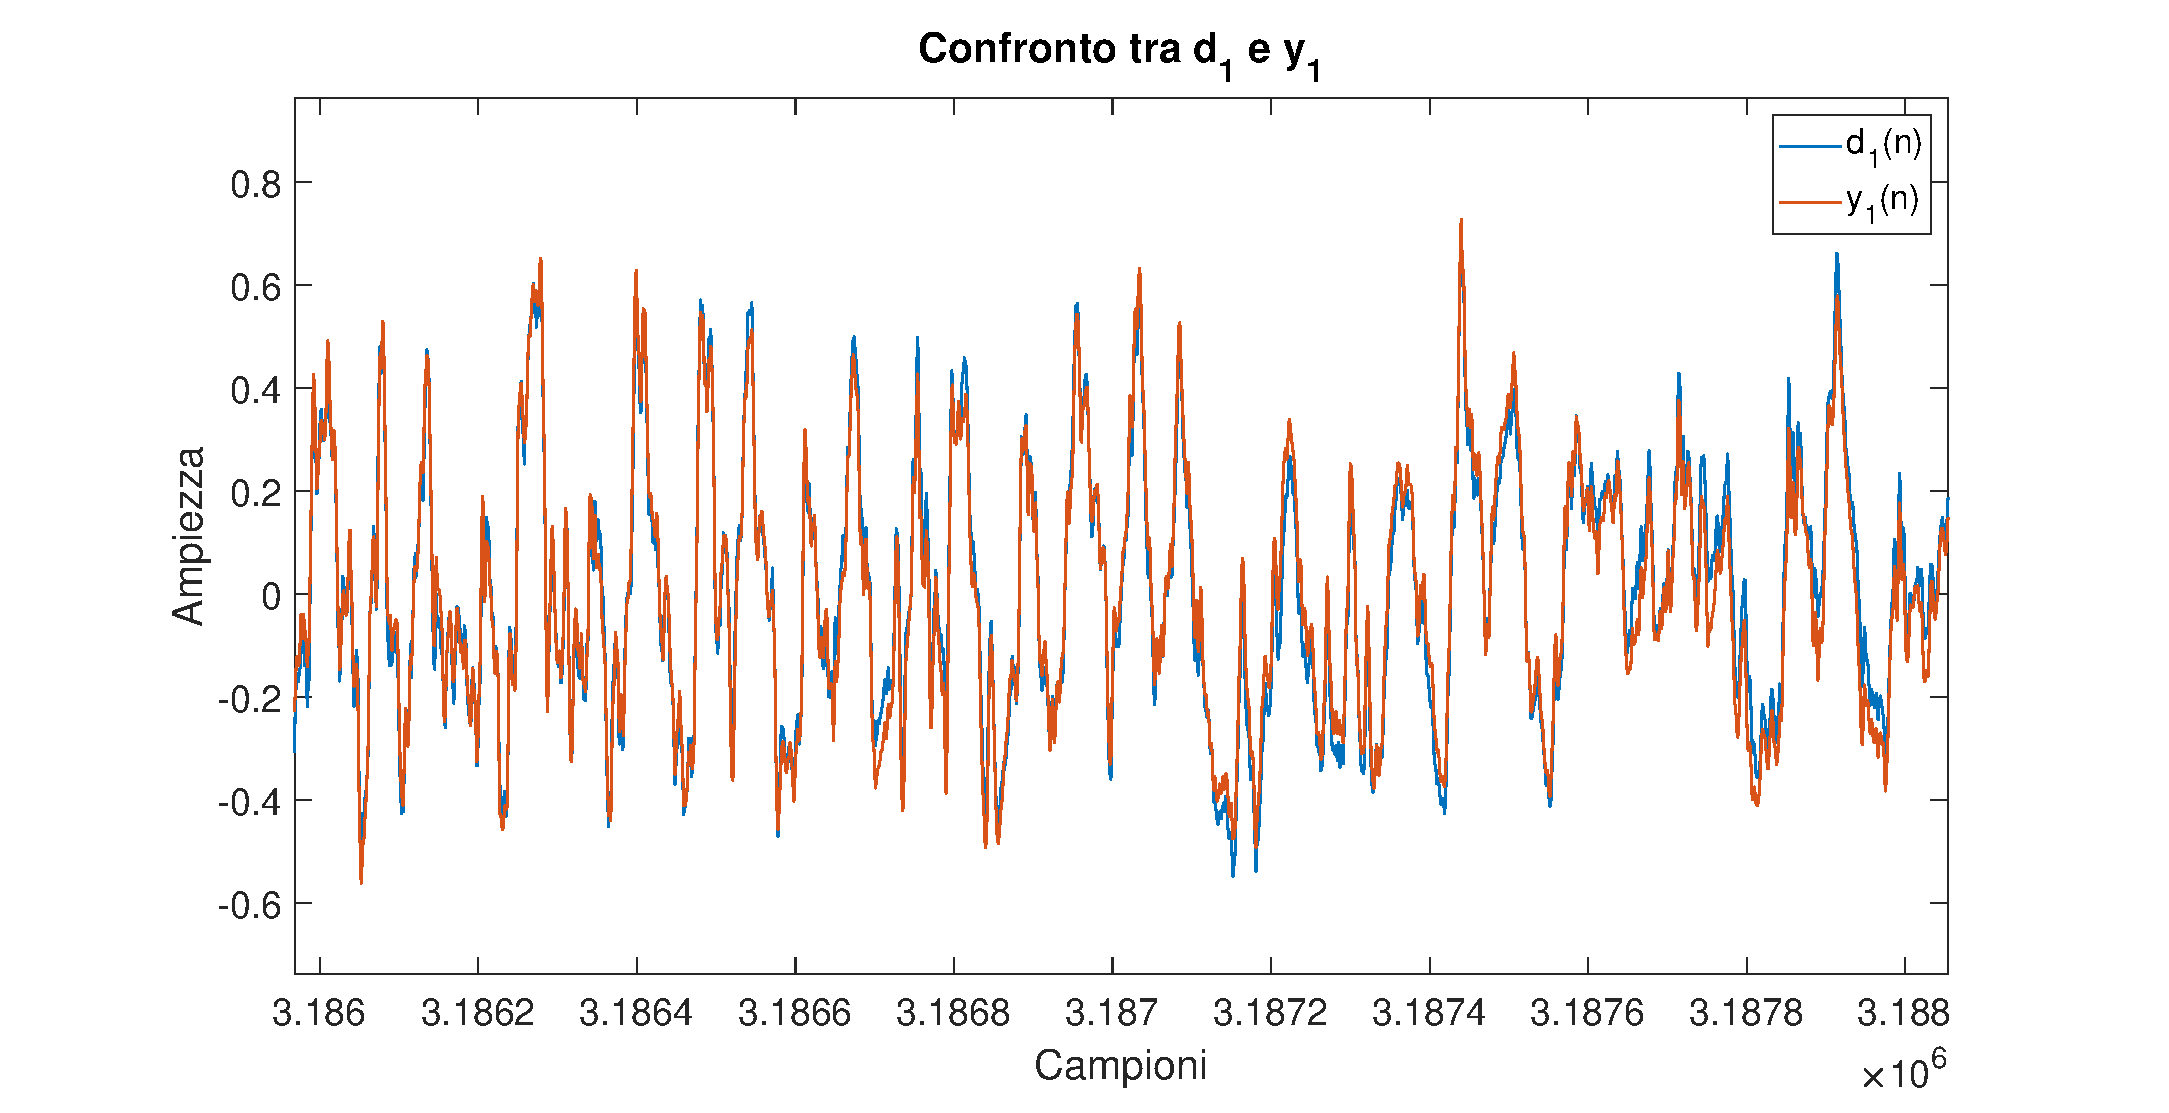
\includegraphics[width=1\textwidth]{Immagini/d1_y1_LMS}
		\caption{}
		\label{fig:d1_y1_LMS}
	\end{subfigure}
	\hfill
	\begin{subfigure}{.45\textwidth}
		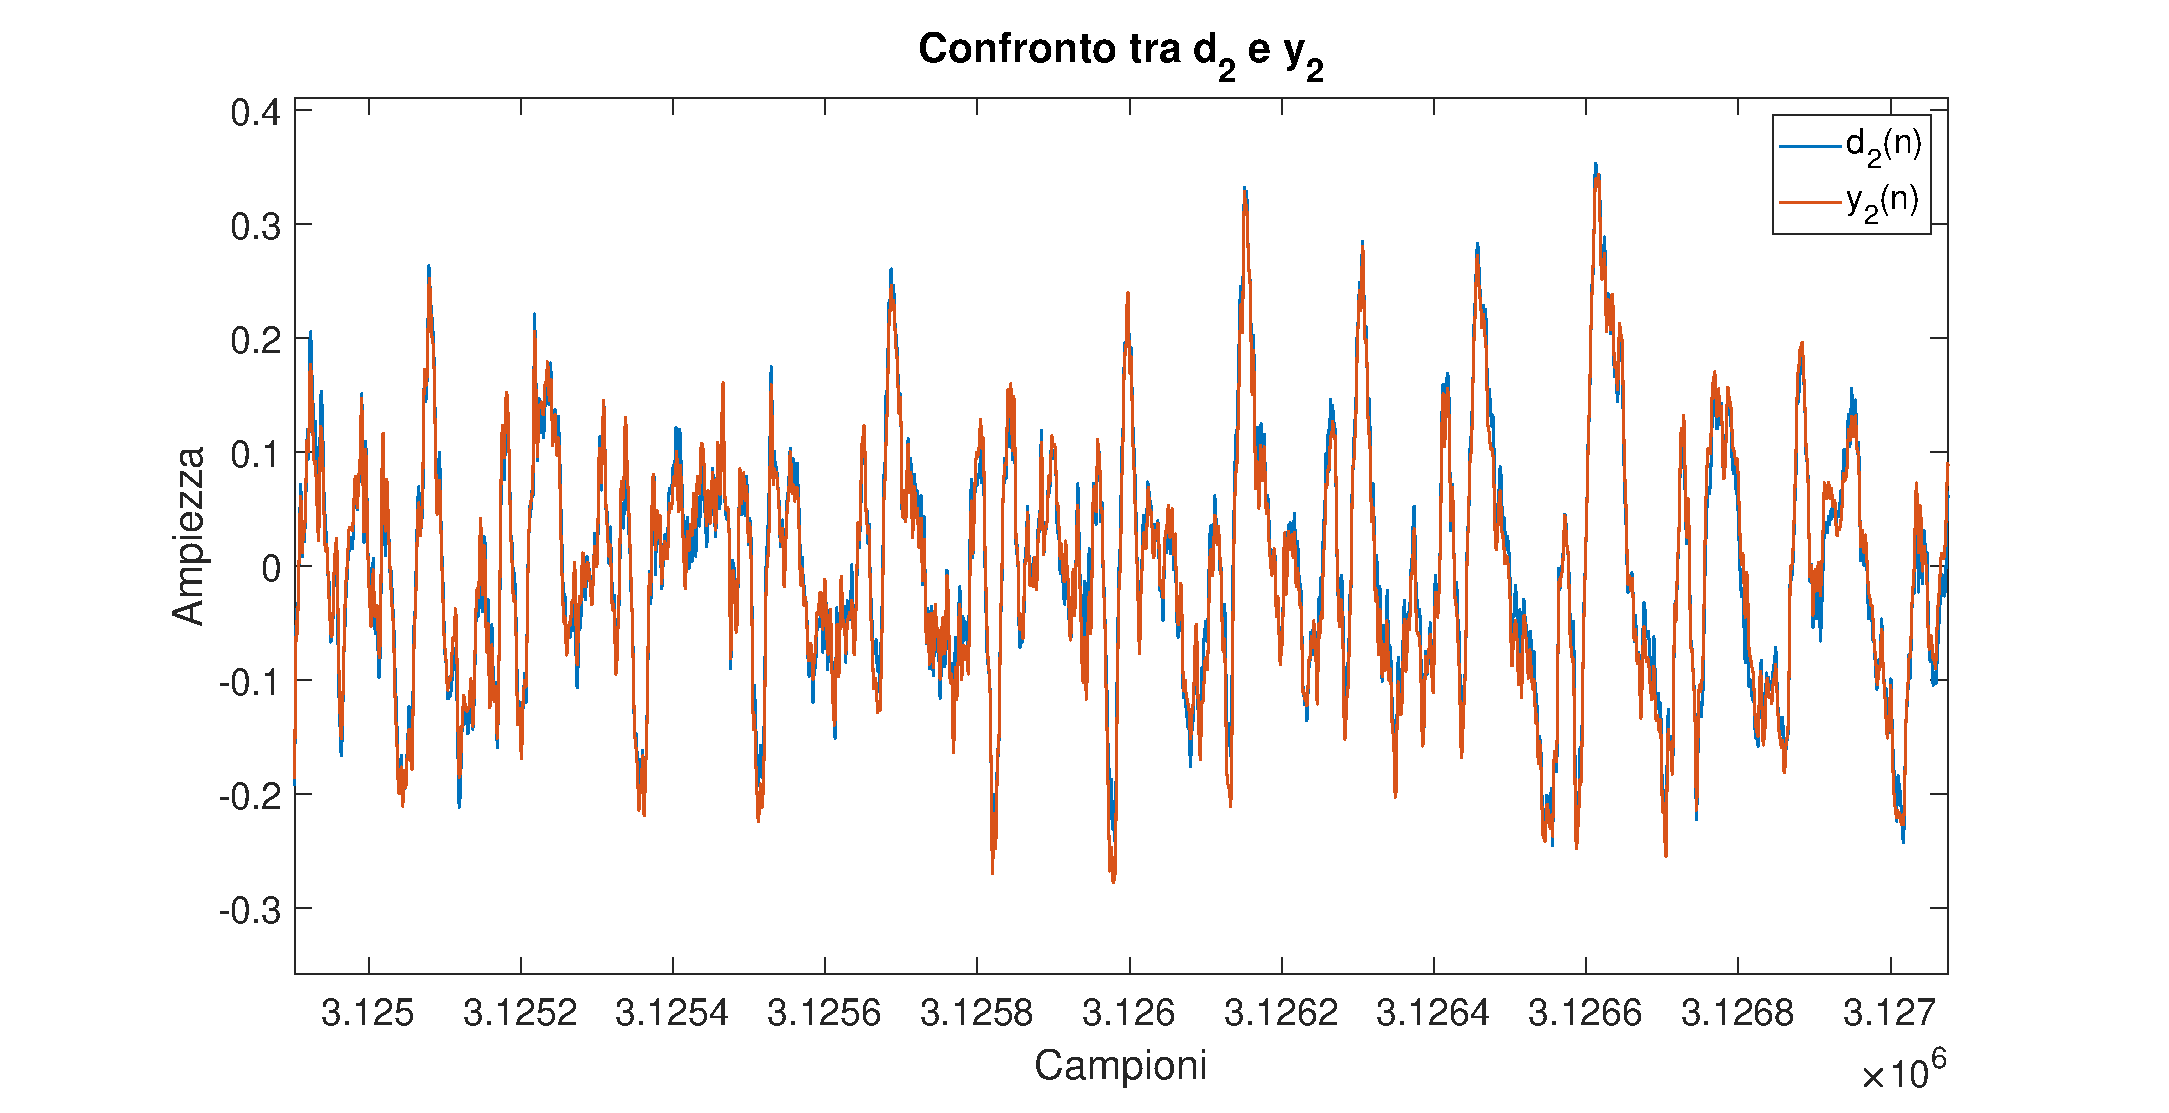
\includegraphics[width=1\textwidth]{Immagini/d2_y2_LMS}
		\caption{}
		\label{fig:d2_y2_LMS}
	\end{subfigure}
	\caption{Confronto degli ingressi e le uscite (a) sinistro e (b) destro della Fast Deconvolution, (c) sinistro e (d) destro di LMS.}
	\label{fig:confronto_ingressi_uscite_LMS_FD}
\end{figure}
\end{frame}

\begin{frame}{Risultati NU-Tech}
\begin{figure}[h]
	\centering
	\begin{subfigure}{.45\textwidth}
		\includegraphics[width=1\textwidth]{Immagini/x1_y1_FD_nutech}
		\caption{}
		\label{fig:x1_y1_FD_nutech}
	\end{subfigure}
	\hfill
	\begin{subfigure}{.45\textwidth}
			\includegraphics[width=1\textwidth]{Immagini/x2_y2_FD_nutech}
			\caption{}
			\label{fig:x2_y2_FD_nutech}
	\end{subfigure}
	\vfill
	\begin{subfigure}{.45\textwidth}
		\includegraphics[width=1\textwidth]{Immagini/d1_y1_LMS_nutech}
		\caption{}
		\label{fig:d1_y1_LMS_nutech}
	\end{subfigure}
	\hfill
	\begin{subfigure}{.45\textwidth}
		\includegraphics[width=1\textwidth]{Immagini/d2_y2_LMS_nutech}
		\caption{}
		\label{fig:d2_y2_LMS_nutech}
	\end{subfigure}
		\caption{Confronto degli ingressi e le uscite (a) sinistro e (b) destro della Fast Deconvolution, (c) sinistro e (d) destro di LMS.}
		\label{fig:confronto_ingressi_uscita_LMS_nutech}
\end{figure}
\end{frame}

\begin{frame}
\begin{figure}[h]
	\centering
	\begin{subfigure}{.45\textwidth}
		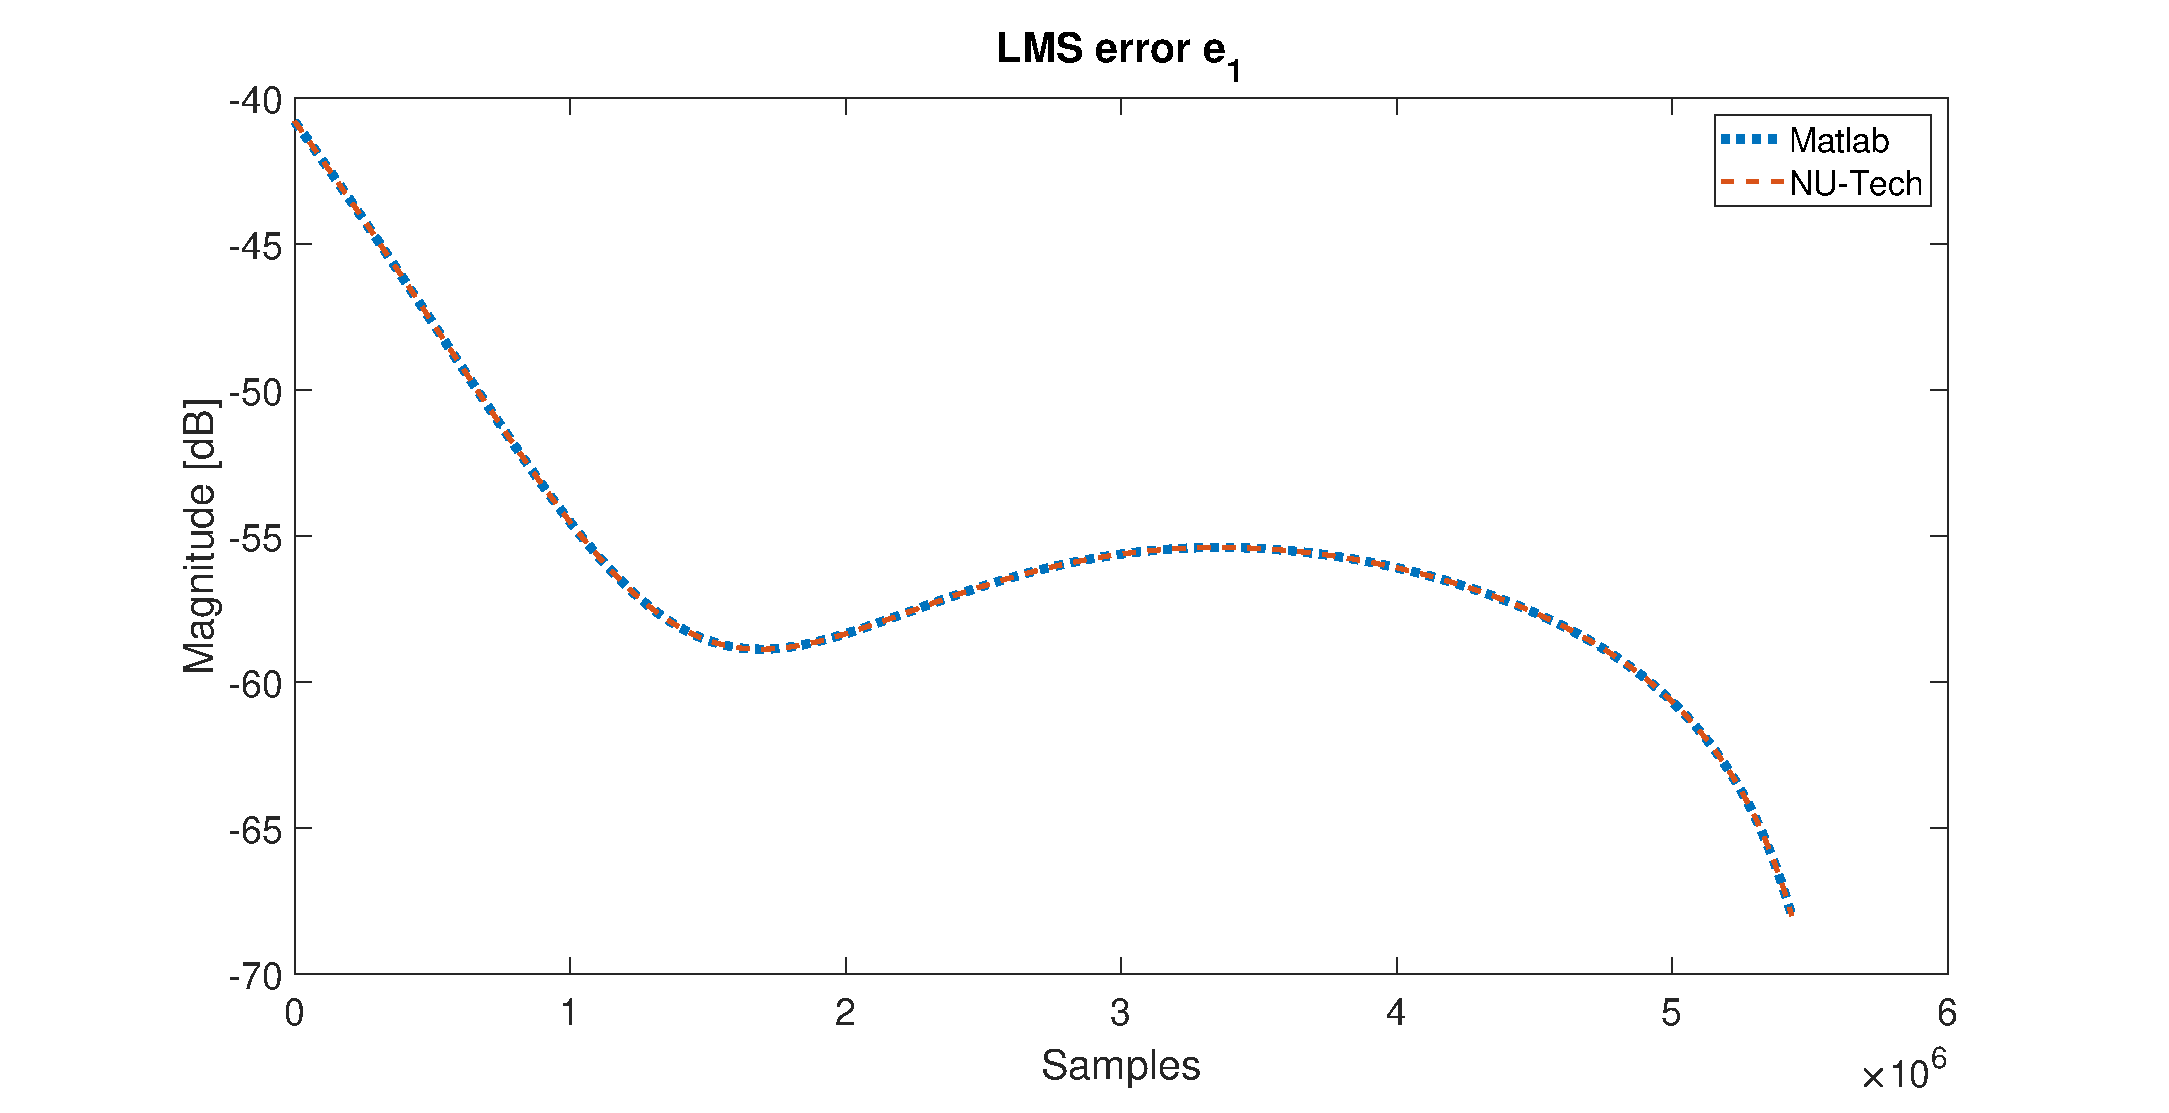
\includegraphics[width=1\textwidth]{Immagini/mse_e1_matlab_nutech}
		\caption{}
		\label{fig:mse_e1_matlab_nutech}
	\end{subfigure}
	\vfill
	\begin{subfigure}{.45\textwidth}
			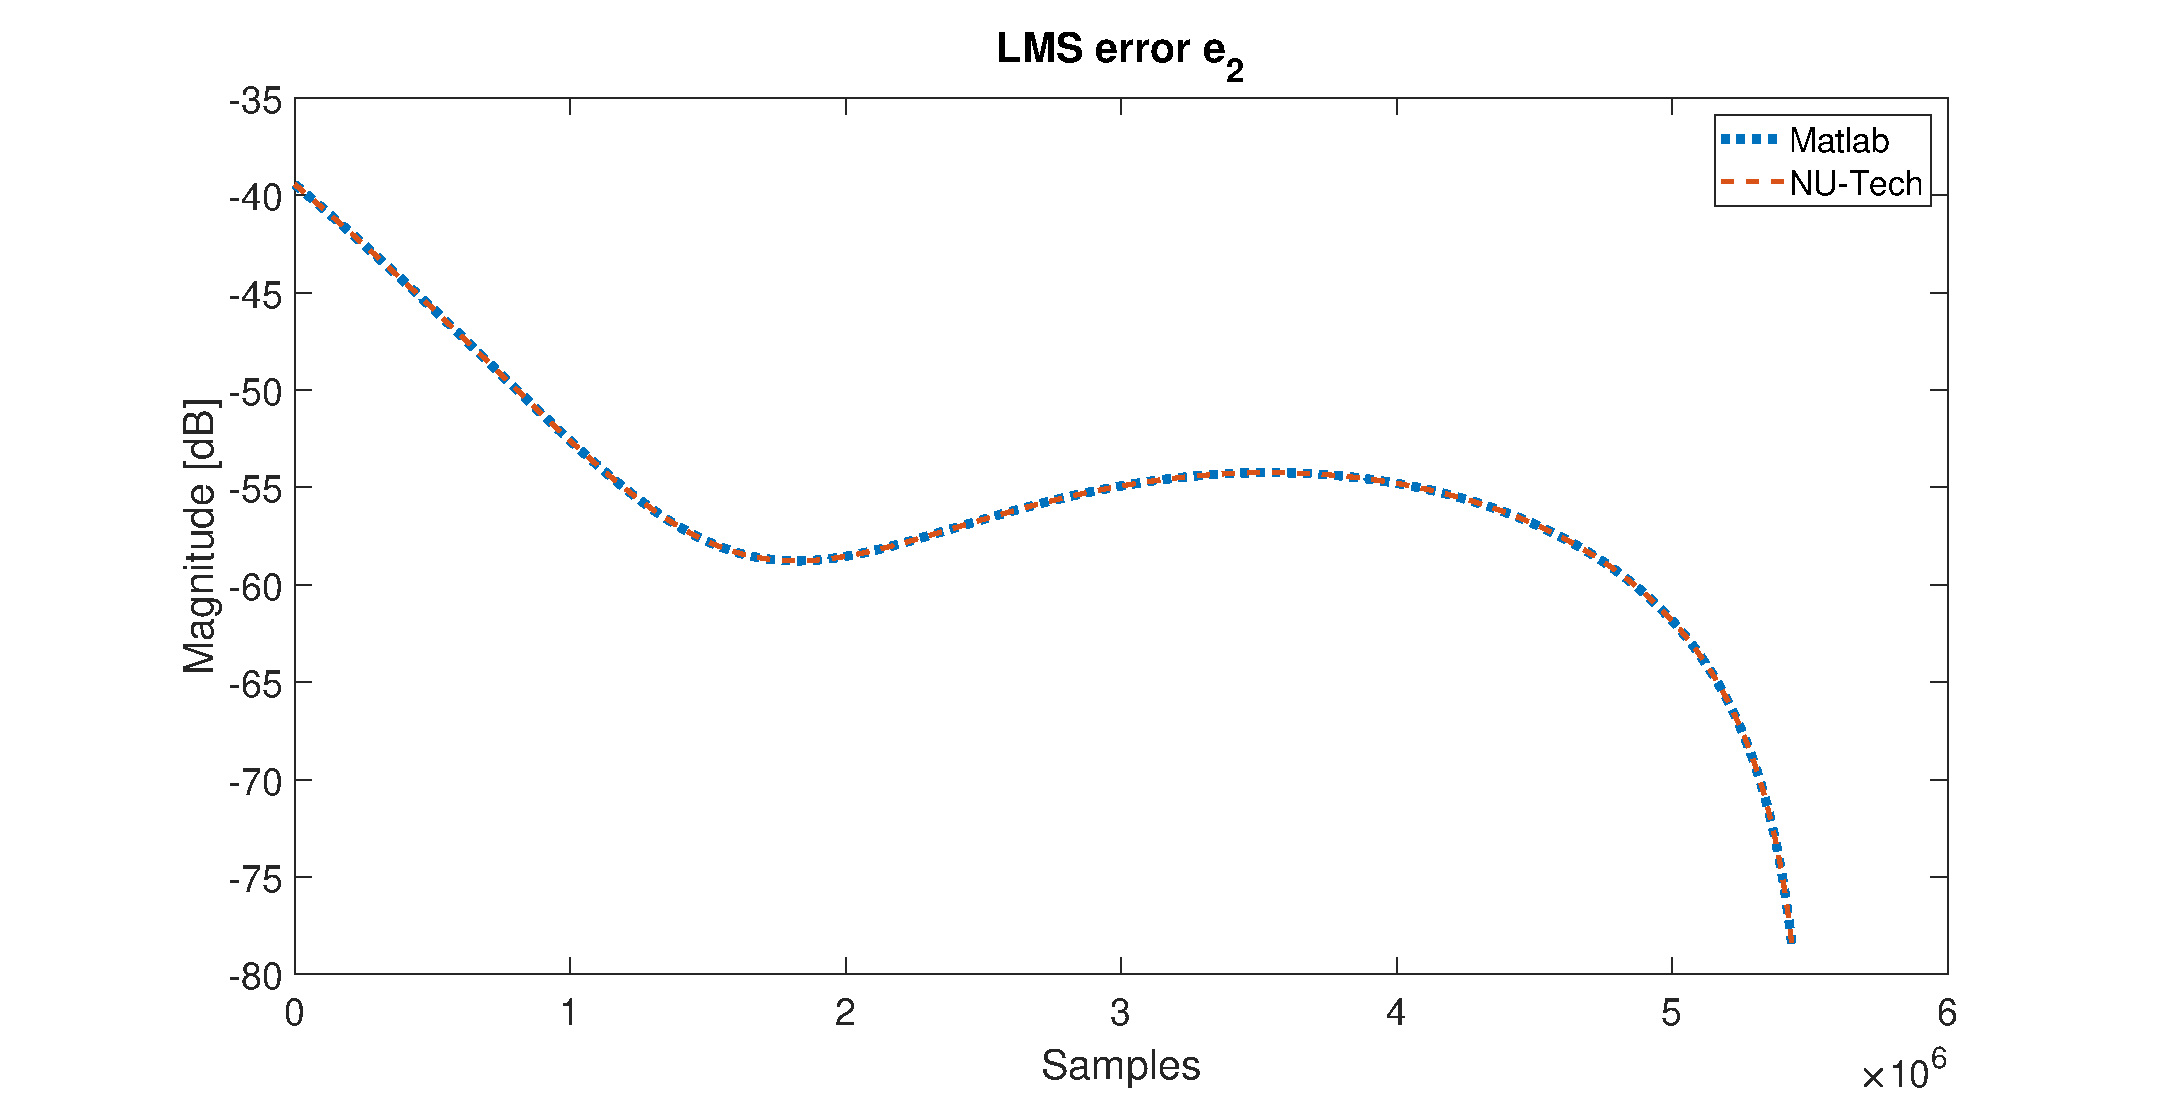
\includegraphics[width=1\textwidth]{Immagini/mse_e2_matlab_nutech}
			\caption{}
			\label{fig:mse_e2_matlab_nutech}
	\end{subfigure}
	\caption{Confronto dell'MSE del canale (a) sinistro e (b) destro dell'algoritmo LMS.}
	\label{fig:mse_matlab_nutech}
\end{figure}
\end{frame}

\begin{frame}
\begin{figure}[h]
	\centering
	\begin{subfigure}{.45\textwidth}
		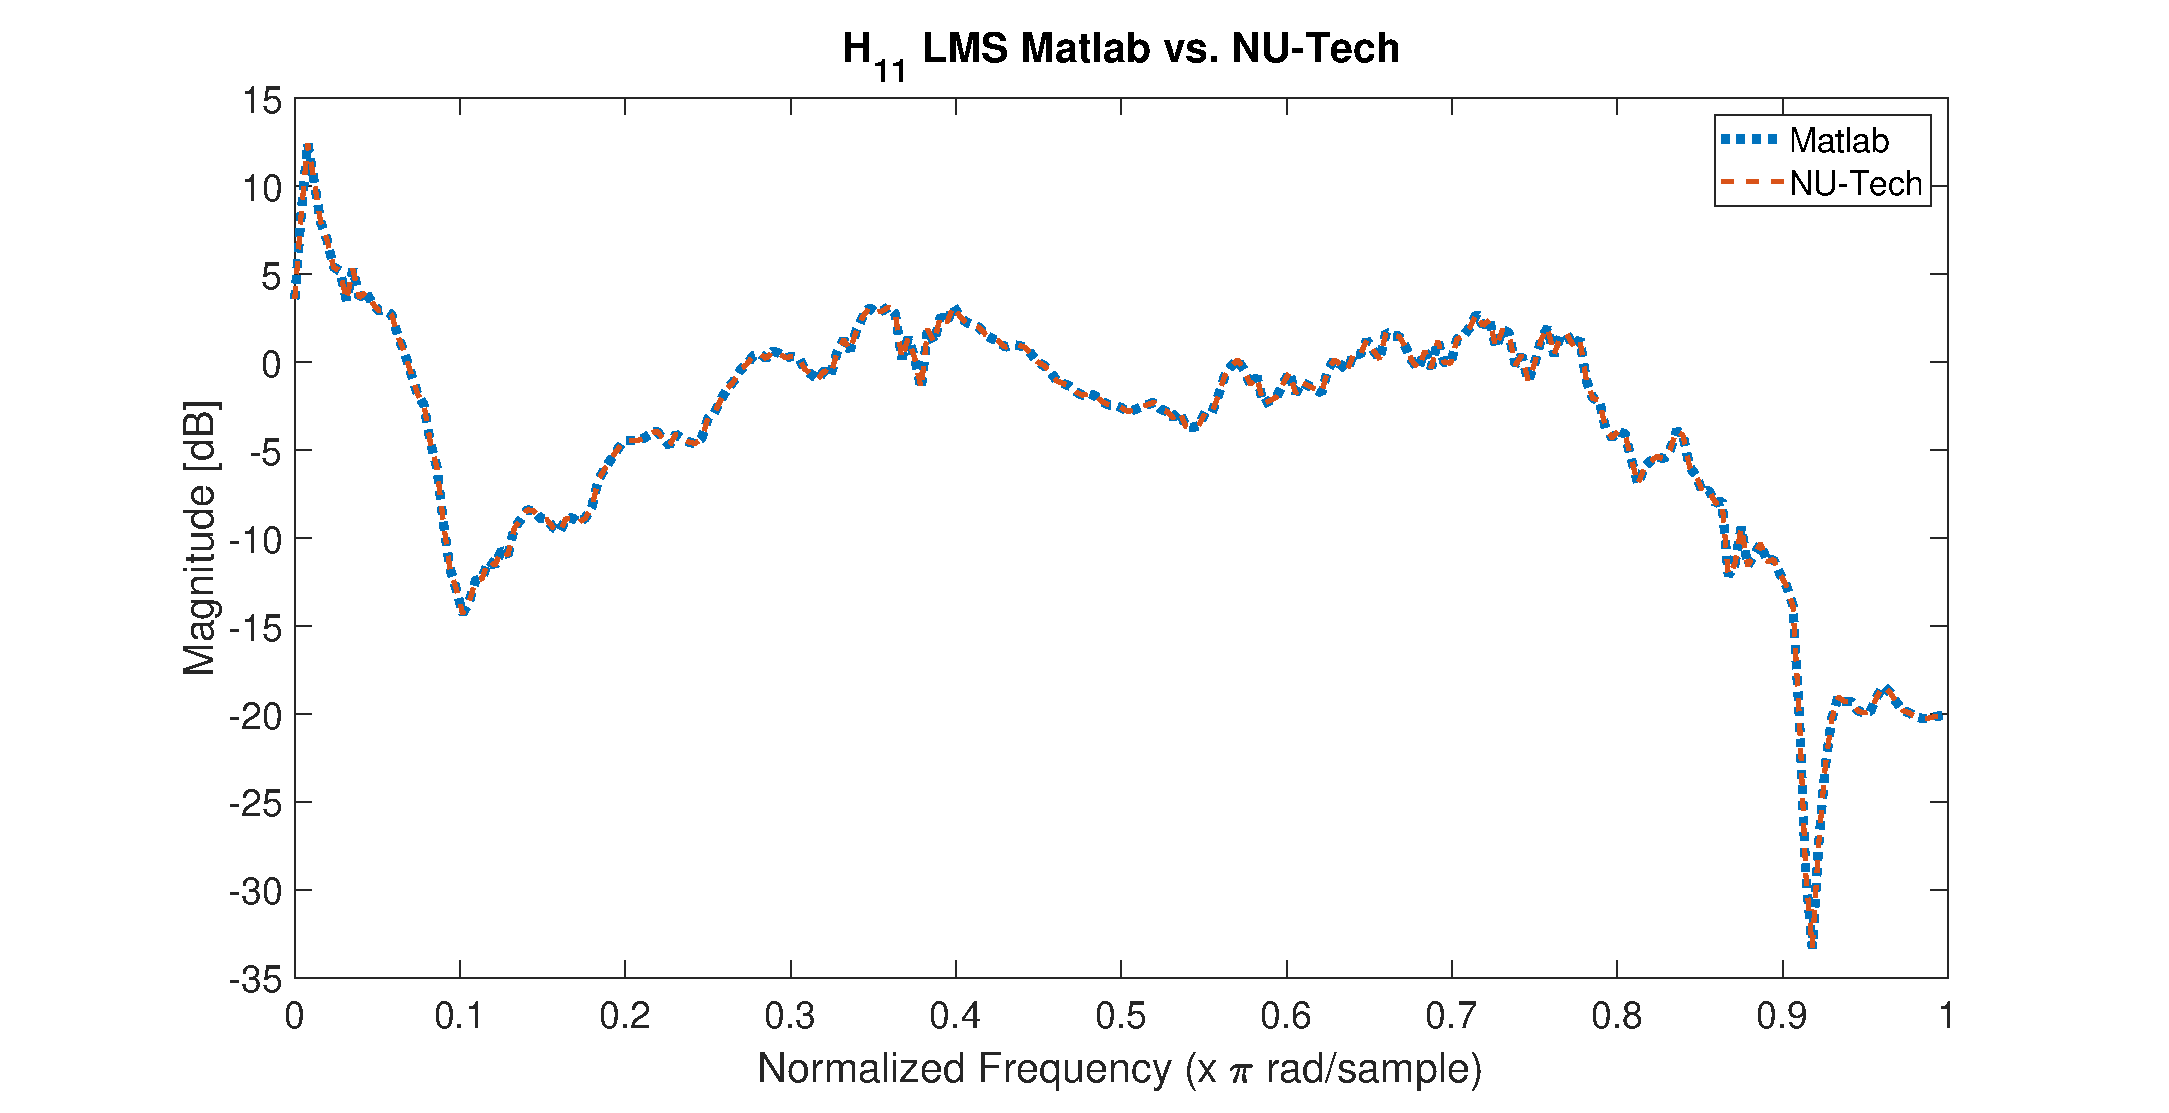
\includegraphics[width=1\textwidth]{Immagini/H11_LMS_matlab_nutech}
		\caption{}
		\label{fig:H11_LMS_matlab_nutech}
	\end{subfigure}
	\hfill
	\begin{subfigure}{.45\textwidth}
			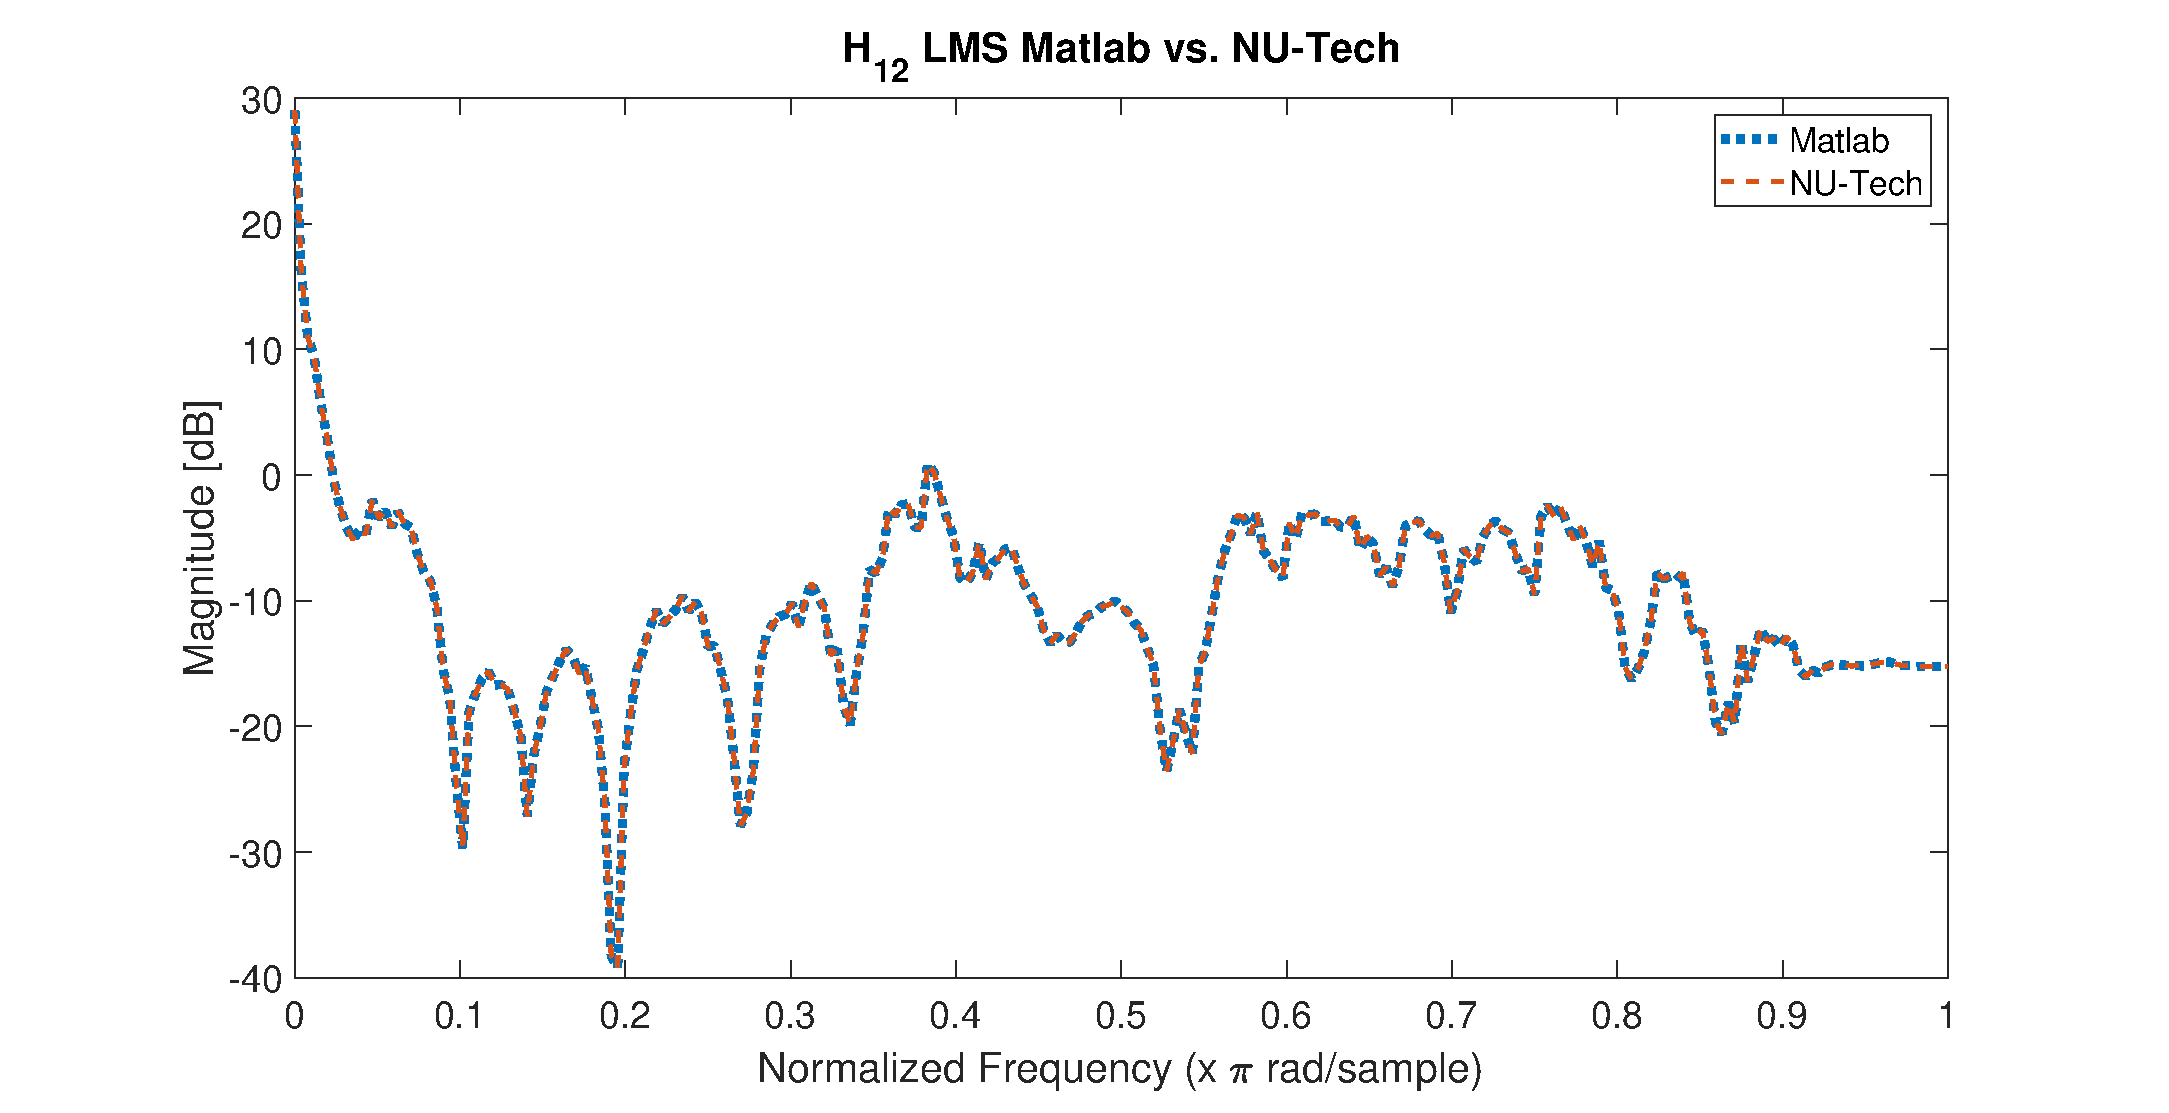
\includegraphics[width=1\textwidth]{Immagini/H12_LMS_matlab_nutech}
			\caption{}
			\label{fig:H12_LMS_matlab_nutech}
	\end{subfigure}
	\vfill
	\begin{subfigure}{.45\textwidth}
		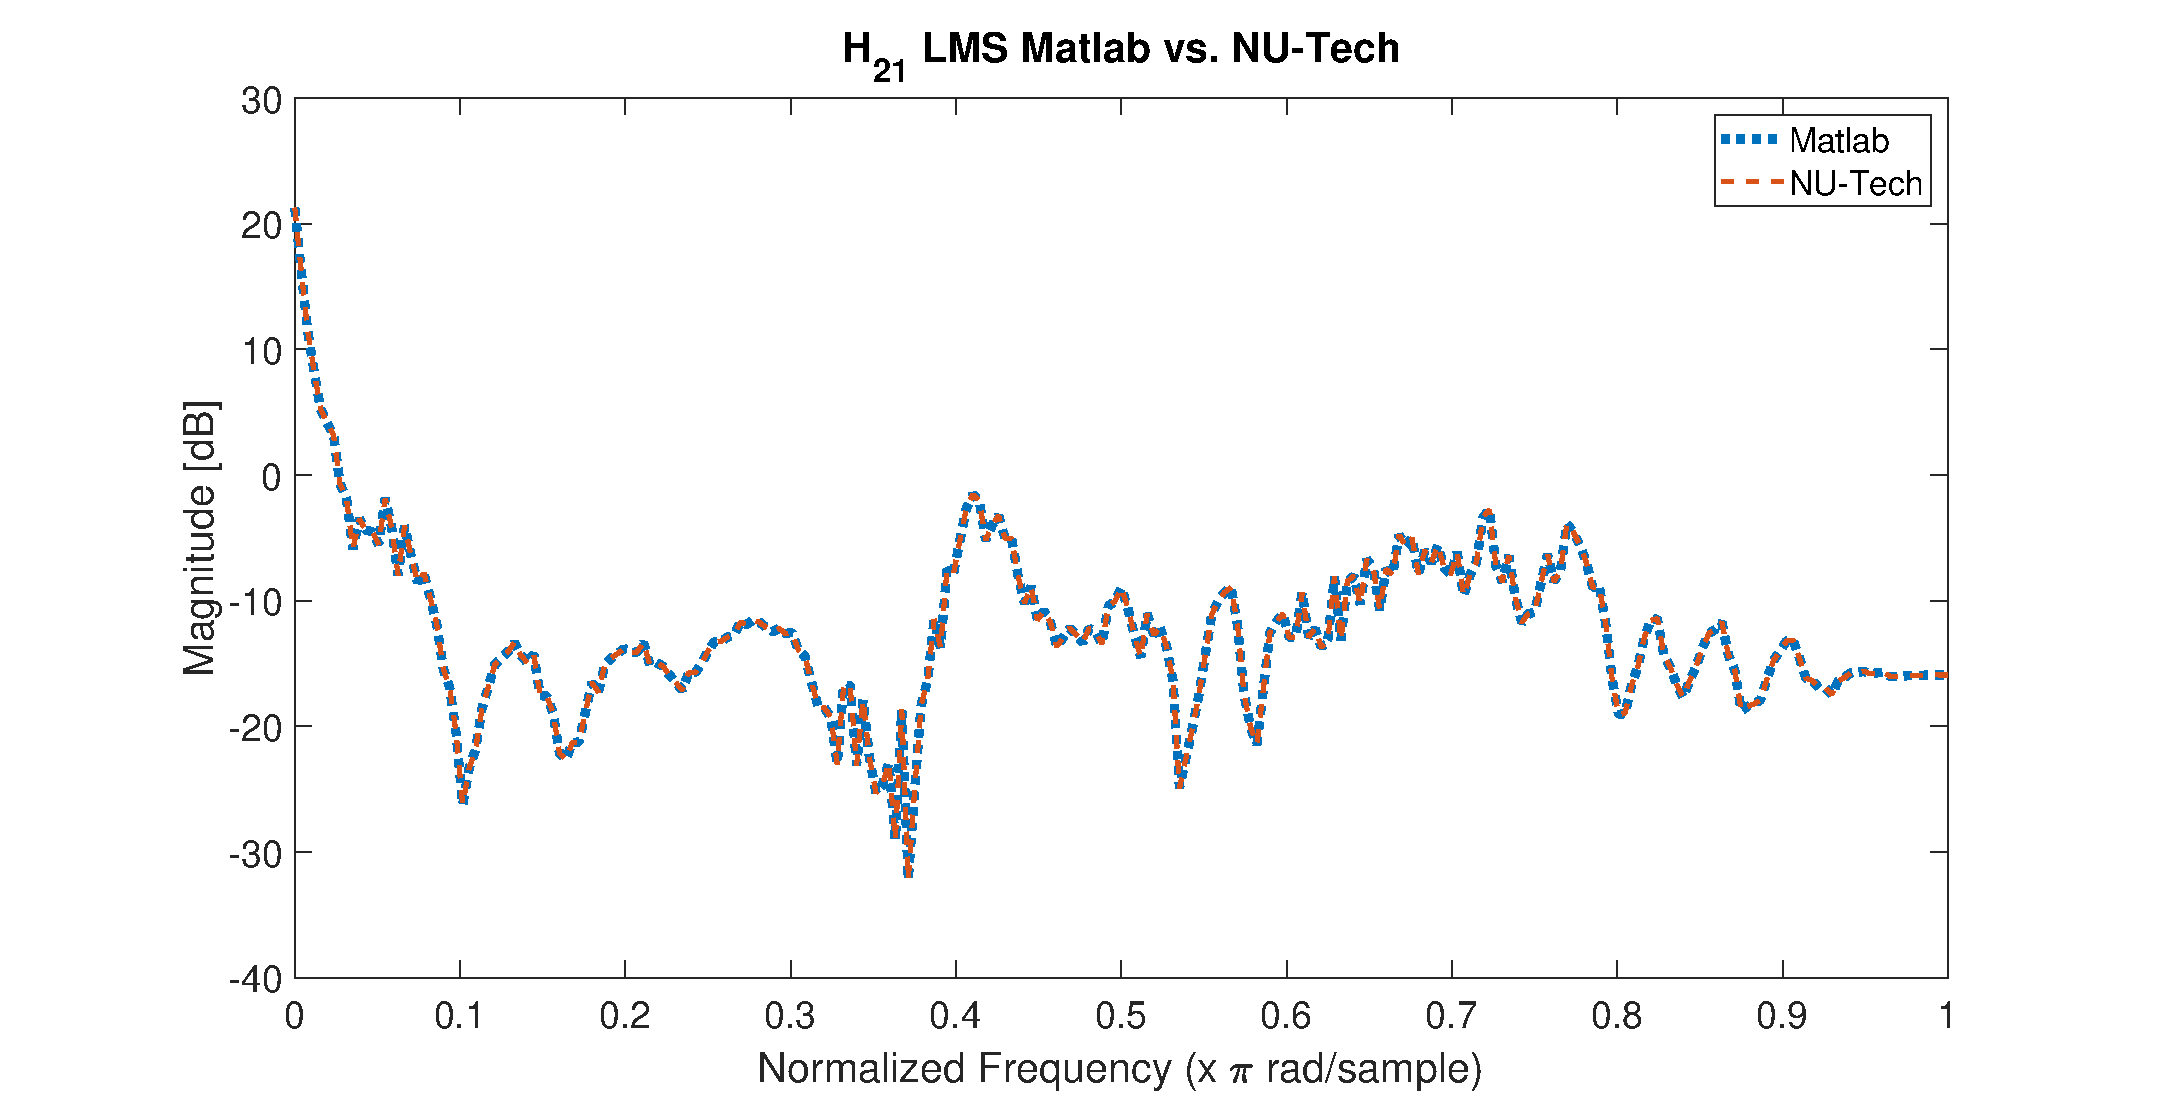
\includegraphics[width=1\textwidth]{Immagini/H21_LMS_matlab_nutech}
		\caption{}
		\label{fig:H21_LMS_matlab_nutech}
	\end{subfigure}
	\hfill
	\begin{subfigure}{.45\textwidth}
		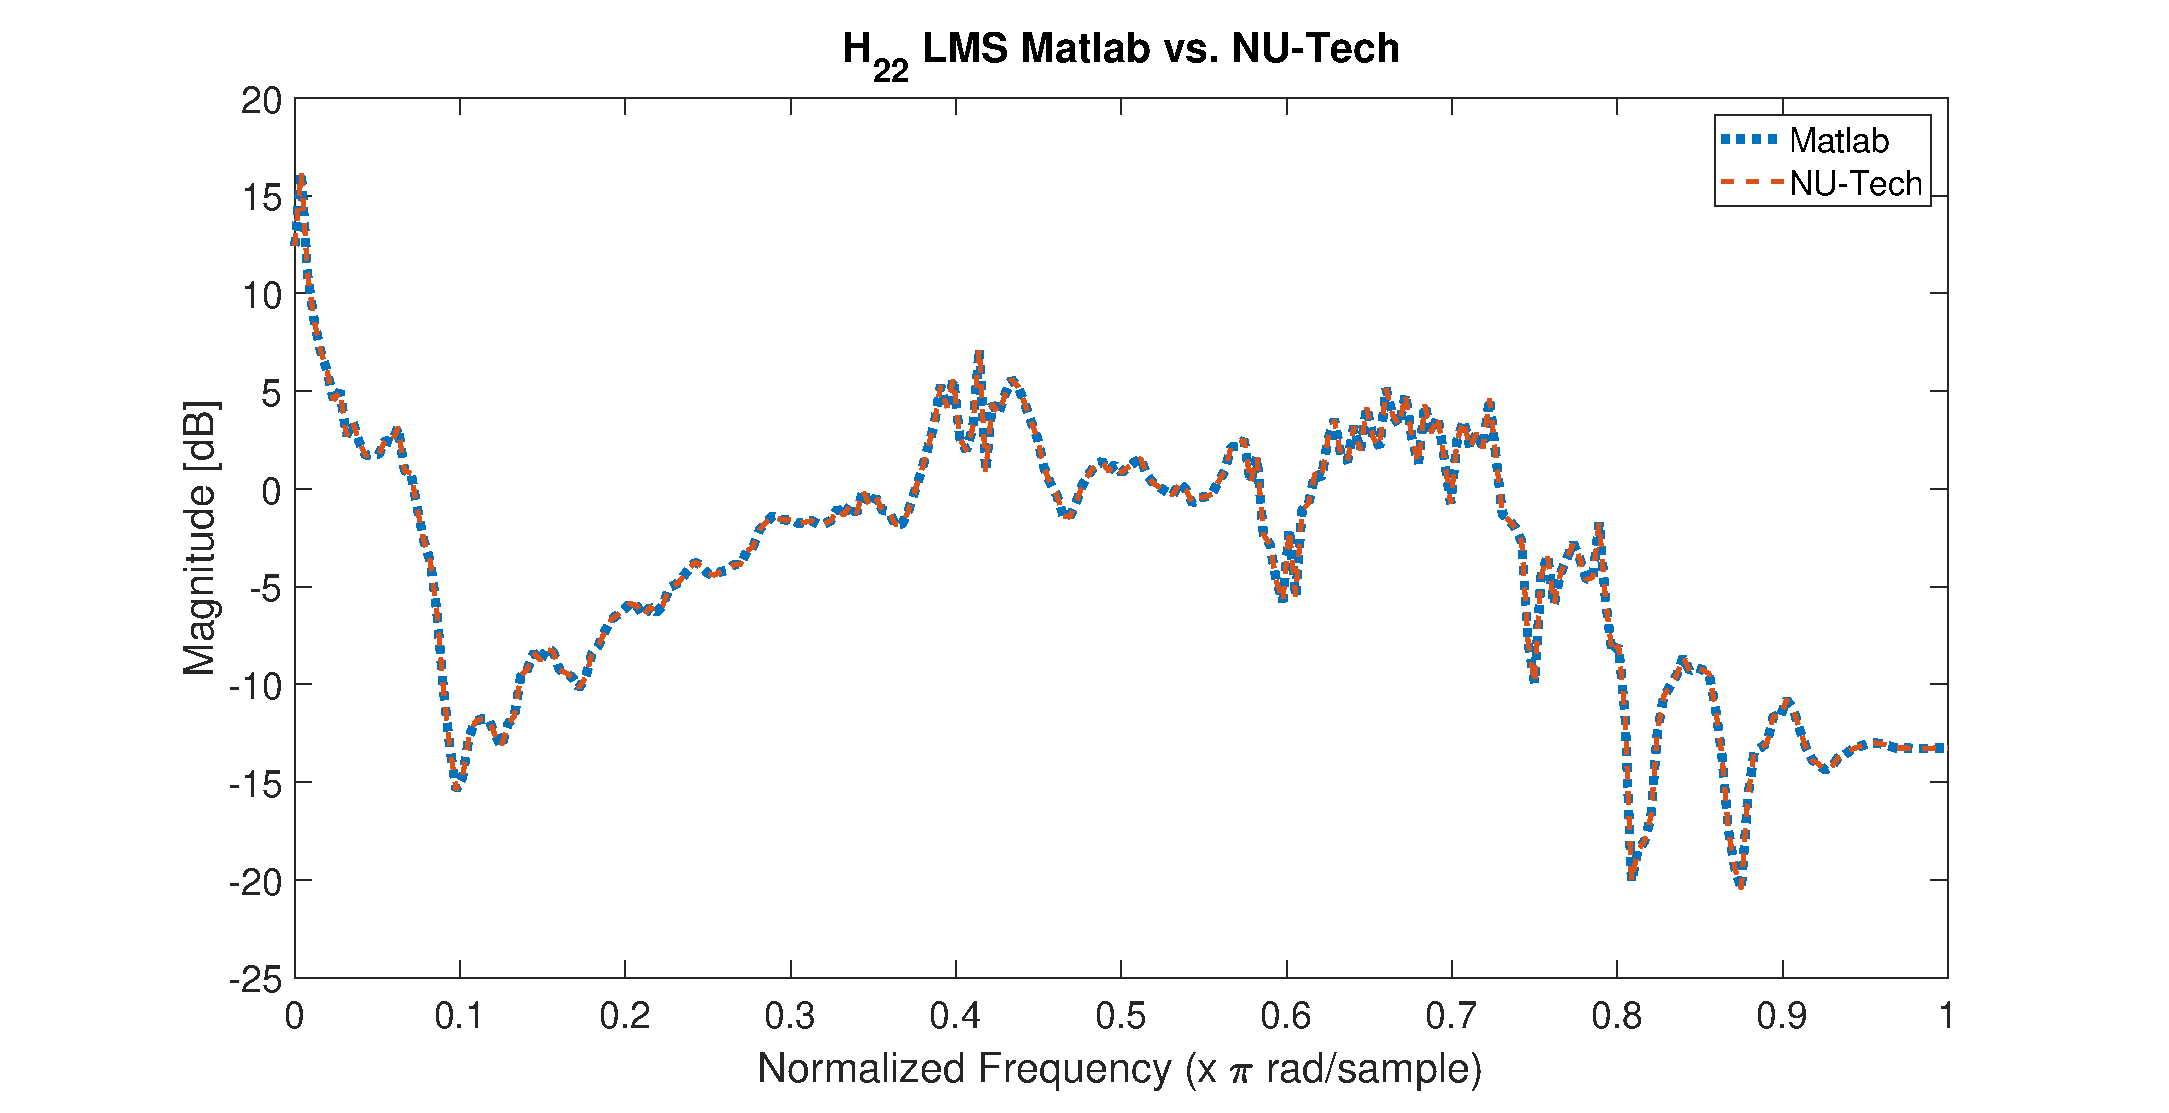
\includegraphics[width=1\textwidth]{Immagini/H22_LMS_matlab_nutech}
		\caption{}
		\label{fig:H22_LMS_matlab_nutech}
	\end{subfigure}
		\caption{Confronto dei filtri di cancellazione del crosstalk (a) $H_{11}$, (b) $H_{12}$, (c) $H_{21}$ e (d) $H_{22}$ in Matlab e in NU-Tech per l'algoritmo LMS.}
		\label{fig:confronto_filtri_matlab_nutech_lms}
\end{figure}
\end{frame}

\begin{frame}
\begin{figure}[h]
	\centering
	\begin{subfigure}{.45\textwidth}
		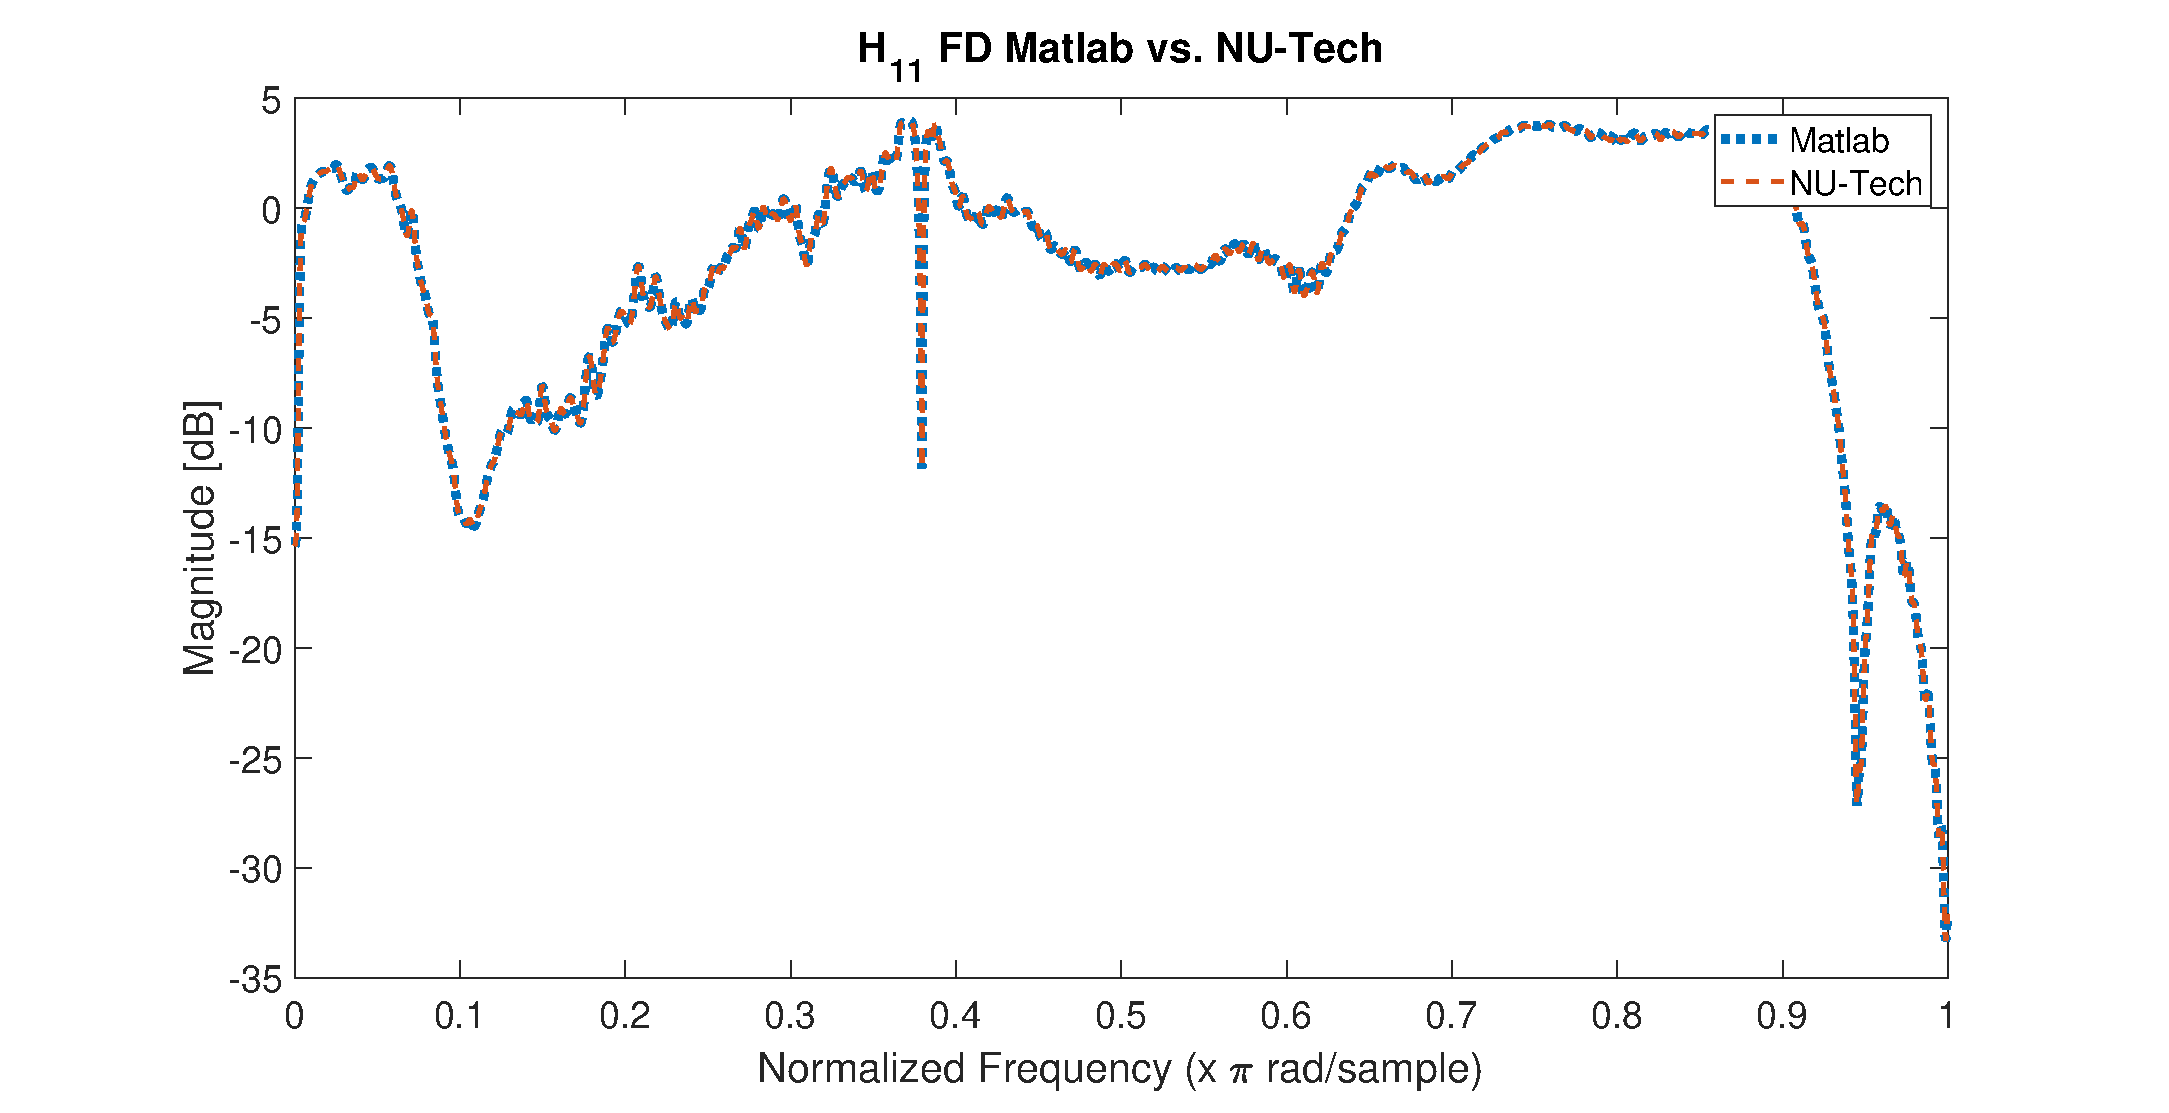
\includegraphics[width=1\textwidth]{Immagini/H11_FD_matlab_nutech}
		\caption{}
		\label{fig:H11_FD_matlab_nutech}
	\end{subfigure}
	\hfill
	\begin{subfigure}{.45\textwidth}
			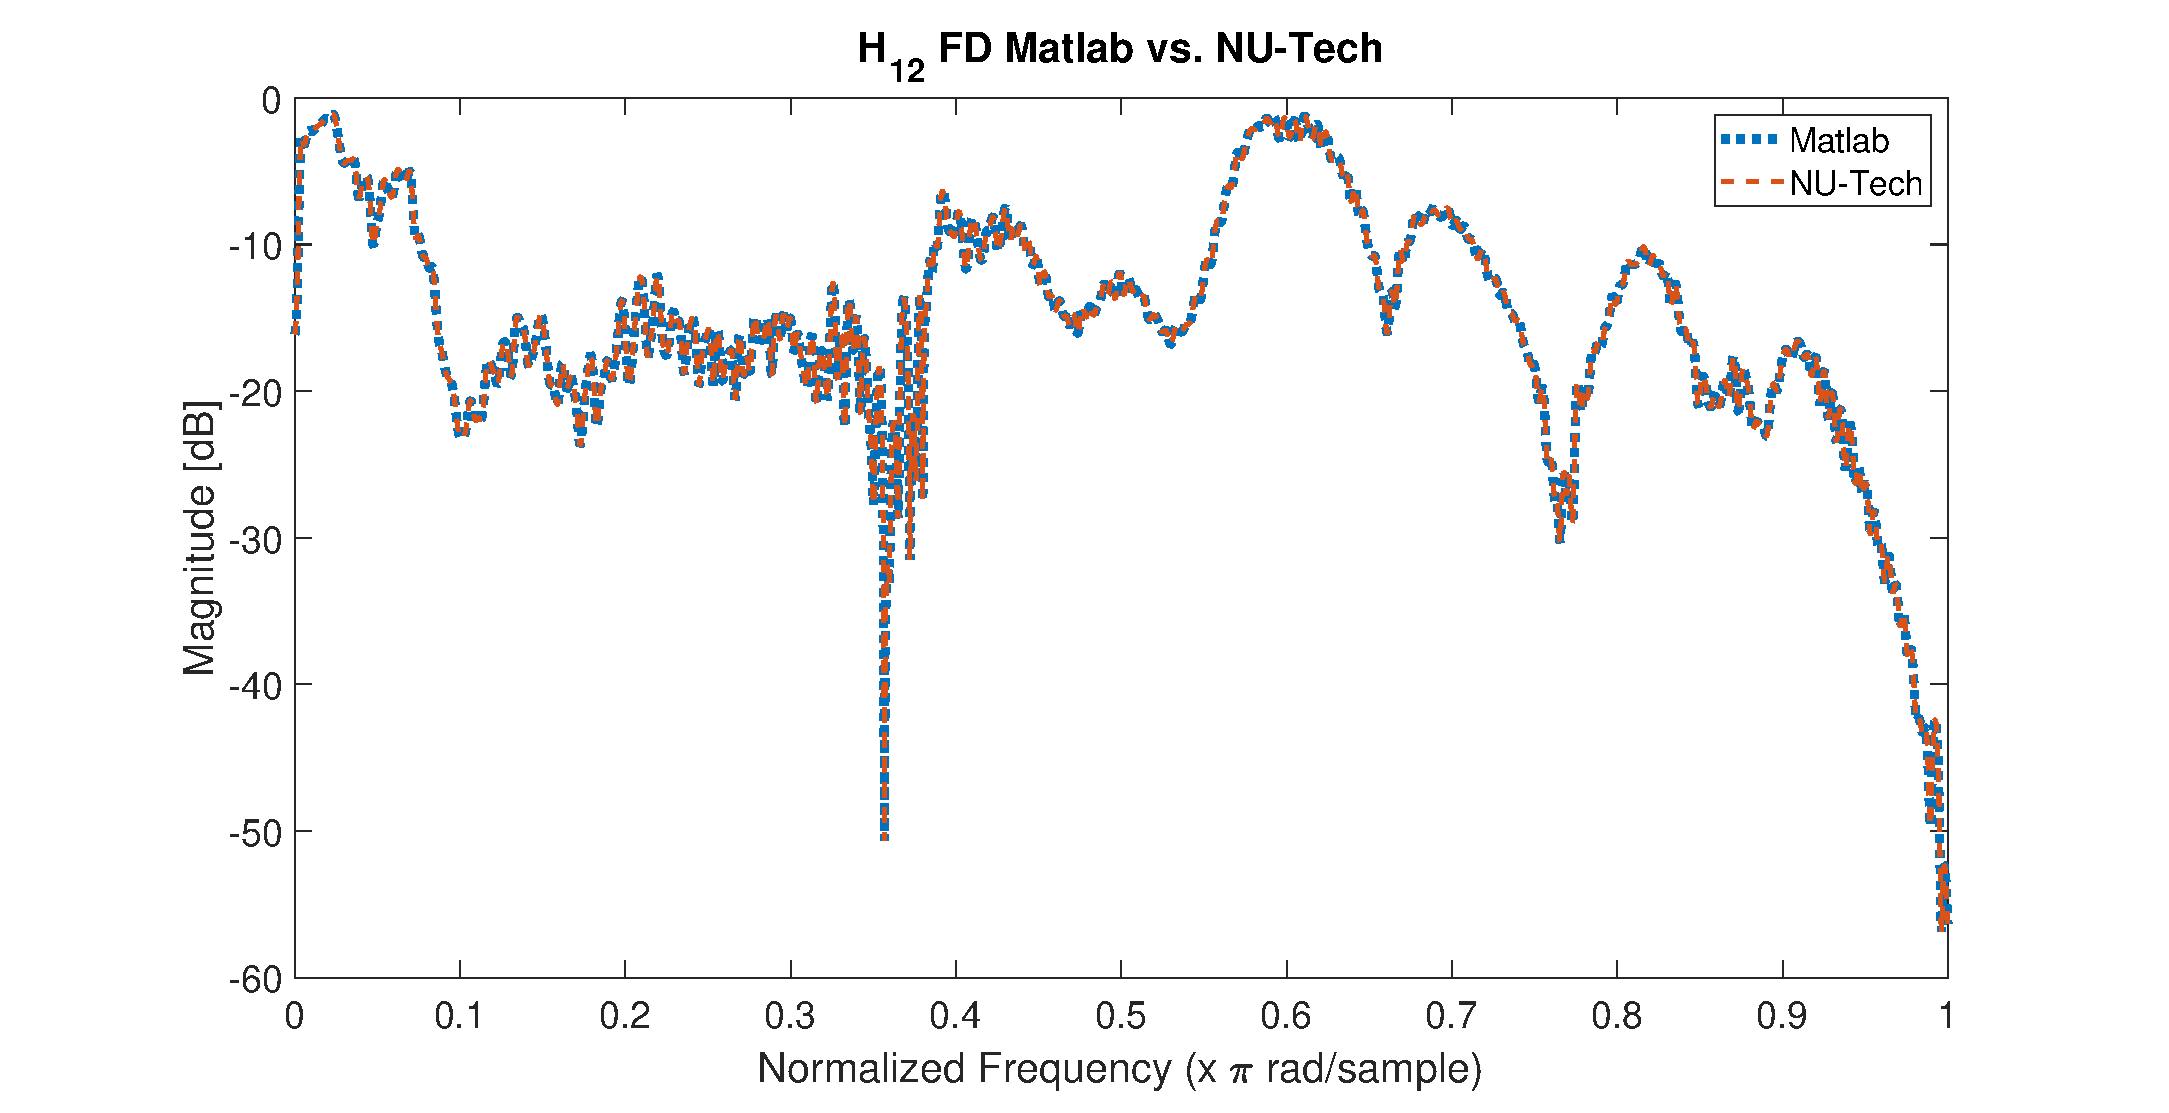
\includegraphics[width=1\textwidth]{Immagini/H12_FD_matlab_nutech}
			\caption{}
			\label{fig:H12_FD_matlab_nutech}
	\end{subfigure}
	\vfill
	\begin{subfigure}{.45\textwidth}
		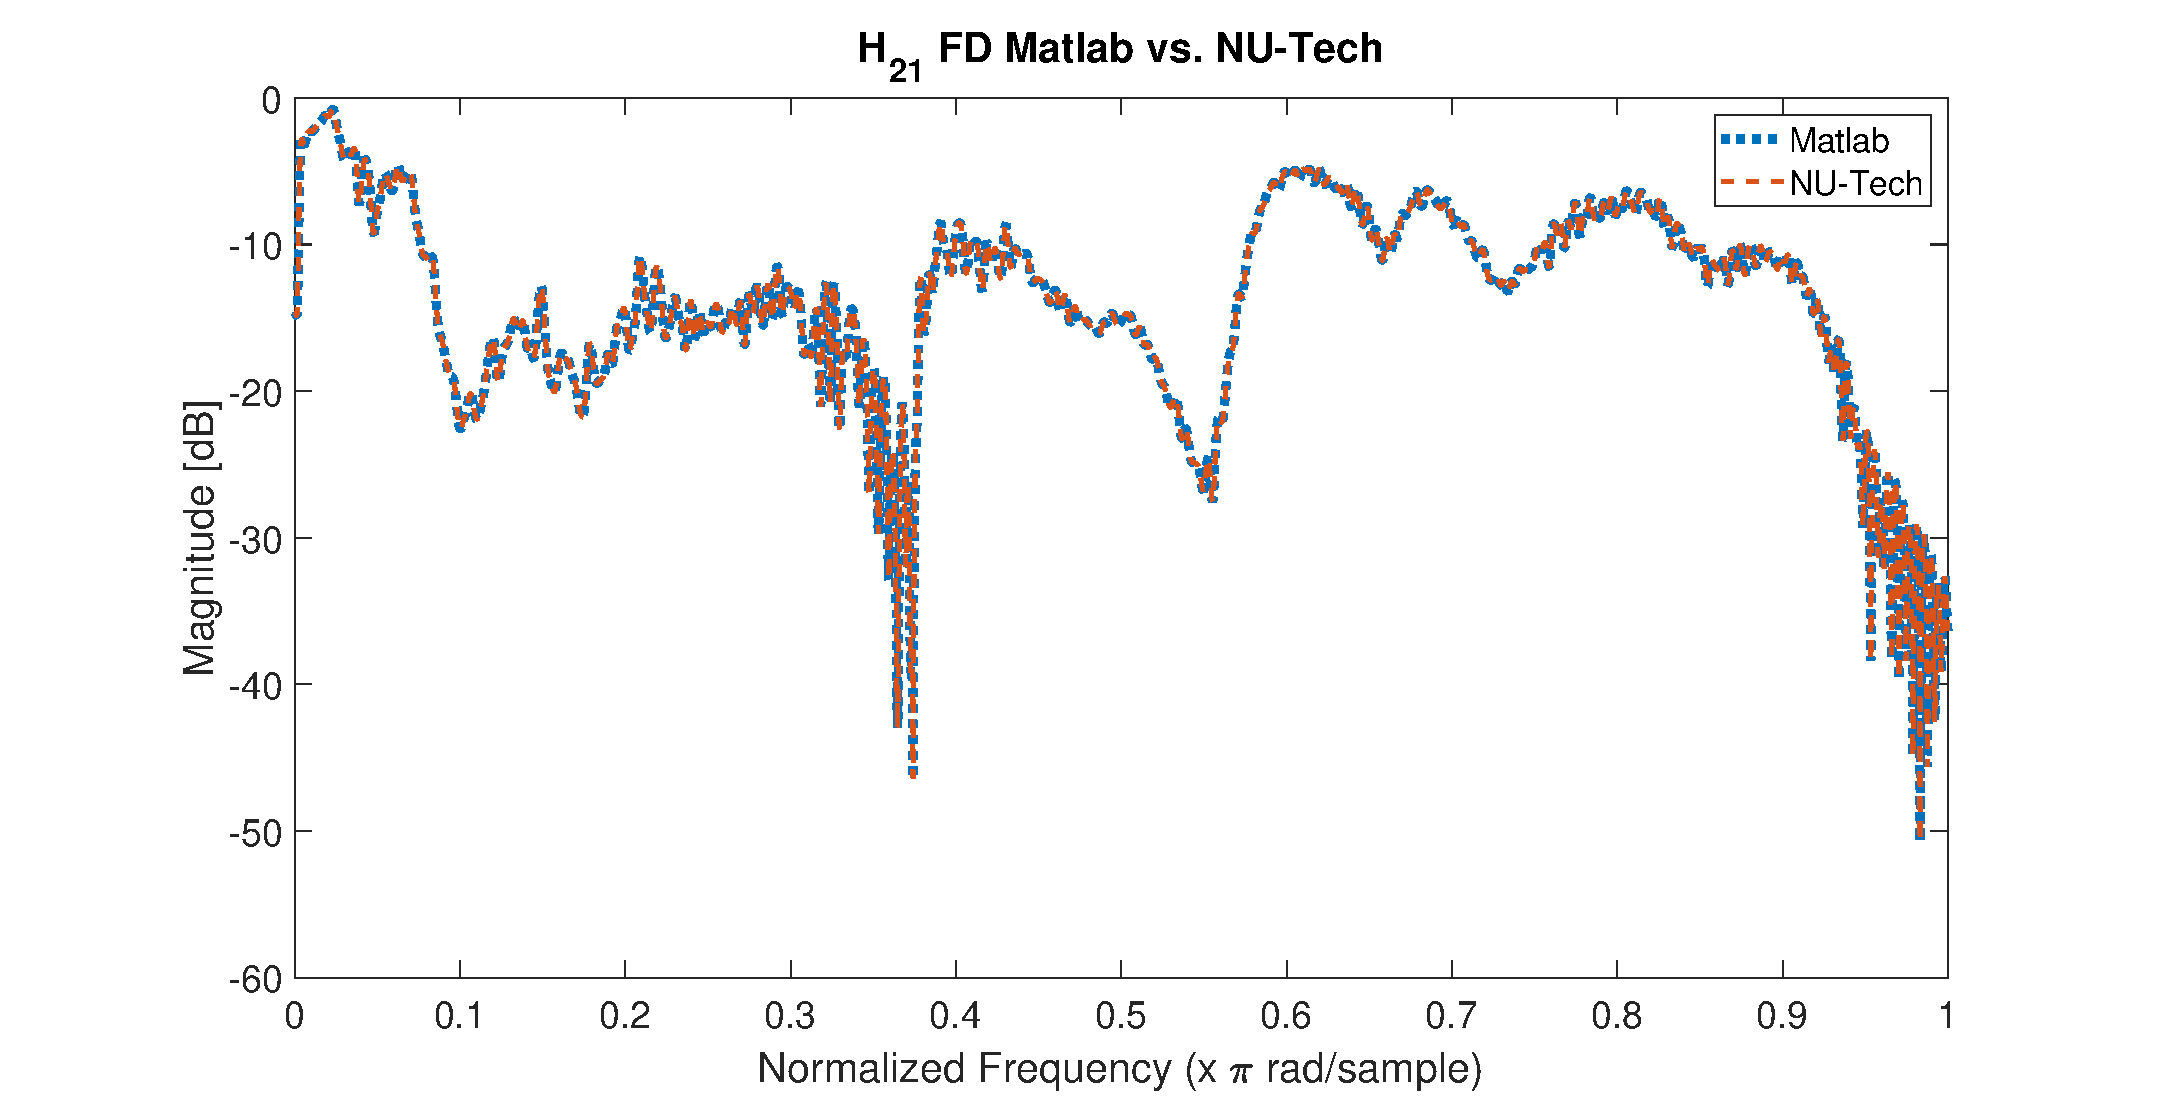
\includegraphics[width=1\textwidth]{Immagini/H21_FD_matlab_nutech}
		\caption{}
		\label{fig:H21_FD_matlab_nutech}
	\end{subfigure}
	\hfill
	\begin{subfigure}{.45\textwidth}
		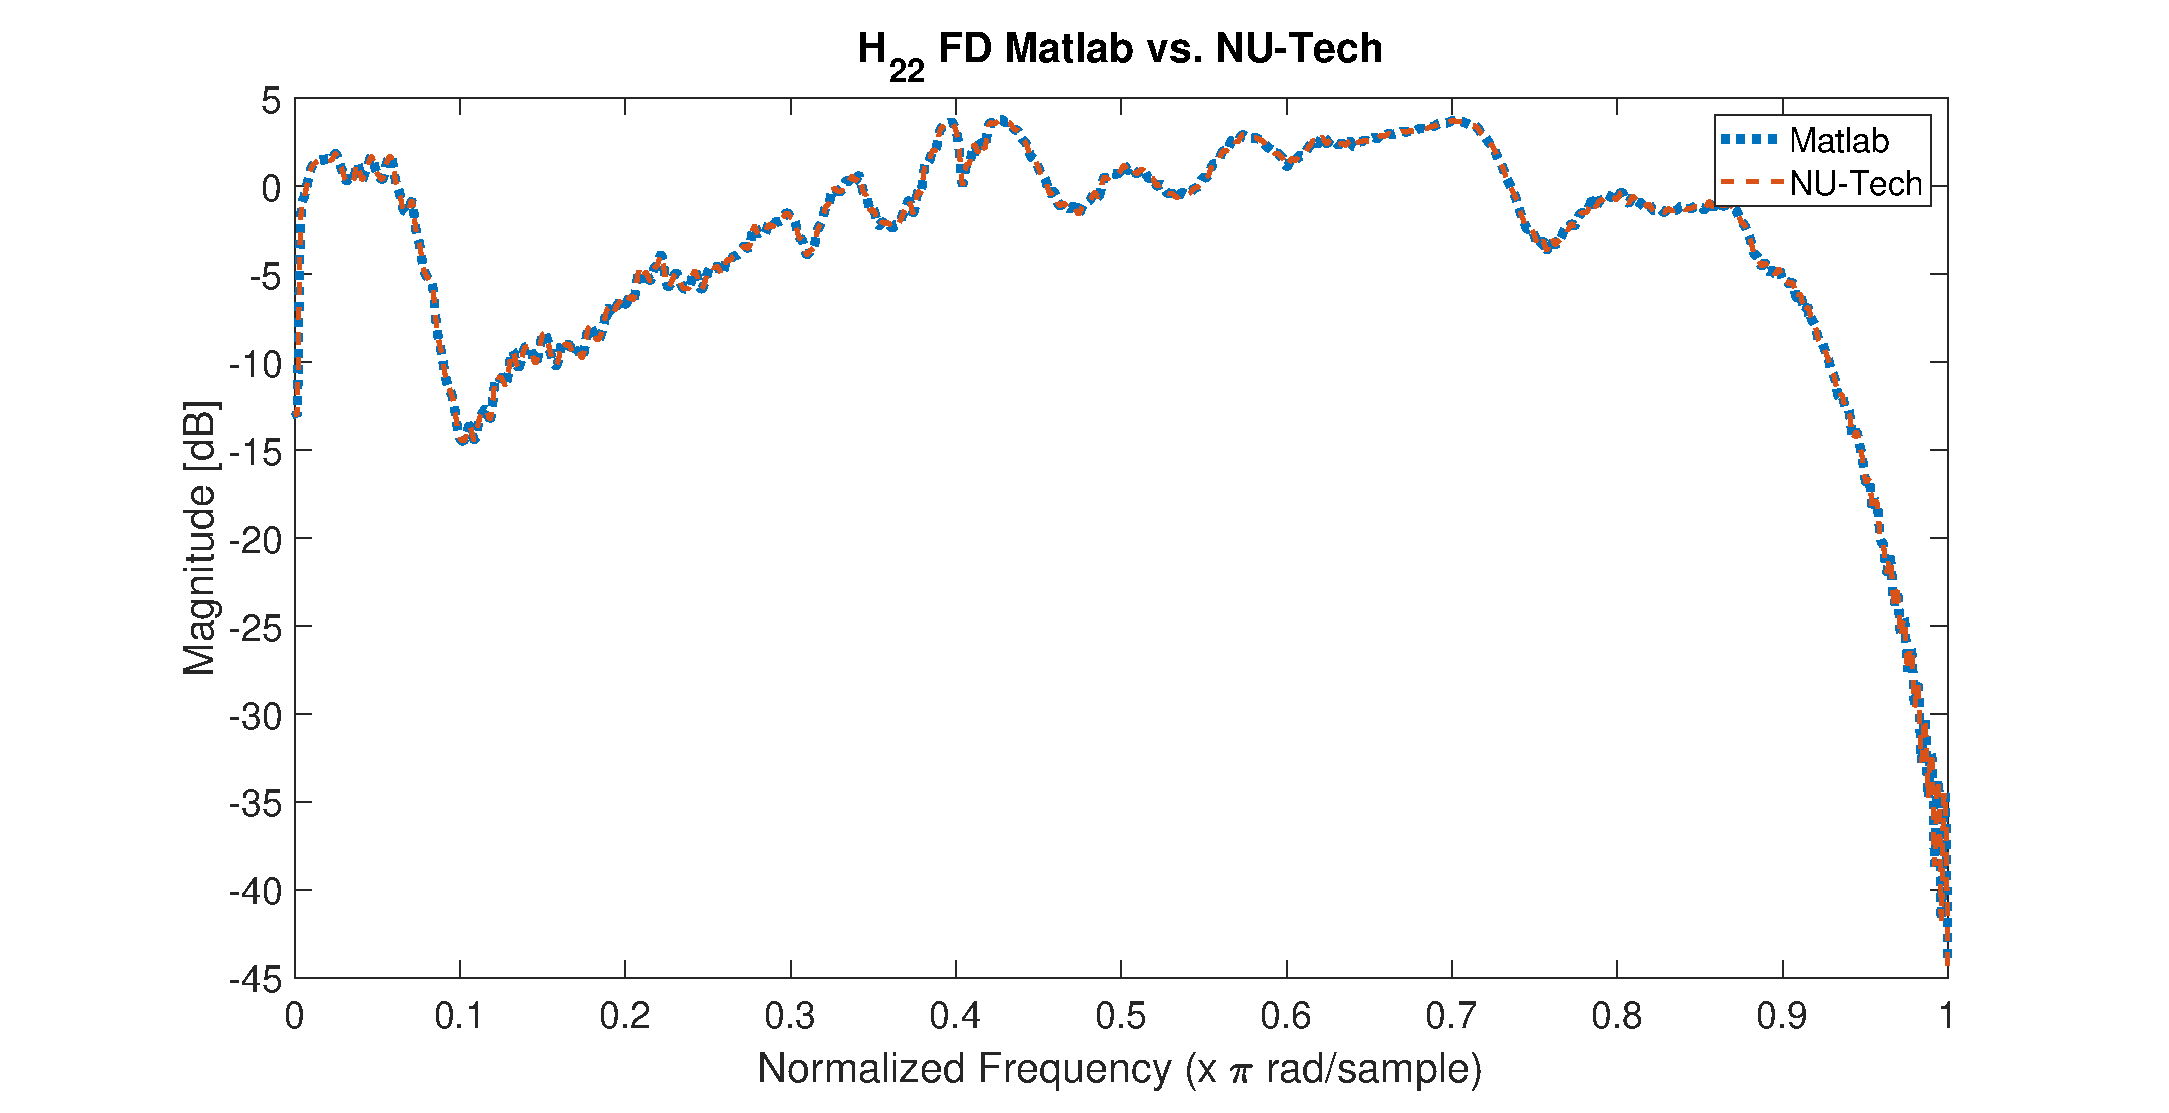
\includegraphics[width=1\textwidth]{Immagini/H22_FD_matlab_nutech}
		\caption{}
		\label{fig:H22_FD_matlab_nutech}
	\end{subfigure}
		\caption{Confronto dei filtri di cancellazione del crosstalk (a) $H_{11}$, (b) $H_{12}$, (c) $H_{21}$ e (d) $H_{22}$ in Matlab e in NU-Tech per l'algoritmo Fast Deconvolution.}
		\label{fig:confronto_filtri_matlab_nutech_fd}
\end{figure}
\end{frame}
\nocite{*}
\section*{Bibliografia}
\begin{frame}[allowframebreaks]
\frametitle{Bibliografia}
\tiny\printbibliography[heading=none]
\end{frame}

\end{document}